% LaTeX Language and campus name and format package
\documentclass[eu,gi]{ifirak}\usepackage[]{graphicx}\usepackage[]{color}
%% maxwidth is the original width if it is less than linewidth
%% otherwise use linewidth (to make sure the graphics do not exceed the margin)
\makeatletter
\def\maxwidth{ %
  \ifdim\Gin@nat@width>\linewidth
    \linewidth
  \else
    \Gin@nat@width
  \fi
}
\makeatother

\definecolor{fgcolor}{rgb}{0.345, 0.345, 0.345}
\newcommand{\hlnum}[1]{\textcolor[rgb]{0.686,0.059,0.569}{#1}}%
\newcommand{\hlstr}[1]{\textcolor[rgb]{0.192,0.494,0.8}{#1}}%
\newcommand{\hlcom}[1]{\textcolor[rgb]{0.678,0.584,0.686}{\textit{#1}}}%
\newcommand{\hlopt}[1]{\textcolor[rgb]{0,0,0}{#1}}%
\newcommand{\hlstd}[1]{\textcolor[rgb]{0.345,0.345,0.345}{#1}}%
\newcommand{\hlkwa}[1]{\textcolor[rgb]{0.161,0.373,0.58}{\textbf{#1}}}%
\newcommand{\hlkwb}[1]{\textcolor[rgb]{0.69,0.353,0.396}{#1}}%
\newcommand{\hlkwc}[1]{\textcolor[rgb]{0.333,0.667,0.333}{#1}}%
\newcommand{\hlkwd}[1]{\textcolor[rgb]{0.737,0.353,0.396}{\textbf{#1}}}%

\usepackage{framed}
\makeatletter
\newenvironment{kframe}{%
 \def\at@end@of@kframe{}%
 \ifinner\ifhmode%
  \def\at@end@of@kframe{\end{minipage}}%
  \begin{minipage}{\columnwidth}%
 \fi\fi%
 \def\FrameCommand##1{\hskip\@totalleftmargin \hskip-\fboxsep
 \colorbox{shadecolor}{##1}\hskip-\fboxsep
     % There is no \\@totalrightmargin, so:
     \hskip-\linewidth \hskip-\@totalleftmargin \hskip\columnwidth}%
 \MakeFramed {\advance\hsize-\width
   \@totalleftmargin\z@ \linewidth\hsize
   \@setminipage}}%
 {\par\unskip\endMakeFramed%
 \at@end@of@kframe}
\makeatother

\definecolor{shadecolor}{rgb}{.97, .97, .97}
\definecolor{messagecolor}{rgb}{0, 0, 0}
\definecolor{warningcolor}{rgb}{1, 0, 1}
\definecolor{errorcolor}{rgb}{1, 0, 0}
\newenvironment{knitrout}{}{} % an empty environment to be redefined in TeX

\usepackage{alltt}

% ERABILIKO DIREN PAKETEAK %

% listings pakage is for code formating
\usepackage{listings}
% Paquete for acents and other special characters
% It is not necesary to use all this packages add or remove those you are interested on
\usepackage[utf8]{inputenc}
\usepackage{colortbl}
\usepackage[table]{xcolor}
\usepackage{graphicx}
\usepackage{wrapfig}
\usepackage{amsfonts}
\usepackage{amsmath}
\usepackage{makeidx}
\usepackage{multicol}
% Definition of colors
\definecolor{darkgreen}{rgb}{0,0.5,0}
\definecolor{lightgray}{rgb}{0.95,0.95,0.95}
\definecolor{gray}{rgb}{0.85,0.85,0.85}
\definecolor{white}{rgb}{1,1,1}
\definecolor{purple}{rgb}{0.51,0,0.25}
\definecolor{orange}{rgb}{0.255,0.178,0.102}
%Definition of style for code
\lstdefinestyle{customc}{
	belowcaptionskip=1\baselineskip,
	breaklines=true,
	tabsize=4,
	language=C,
	showstringspaces=false,
	basicstyle=\footnotesize\ttfamily,
	keywordstyle=\bfseries\color{darkgreen},
	commentstyle=\itshape\color{purple},
	identifierstyle=\color{black},
	stringstyle=\color{orange},
	backgroundcolor=\color{white},
}
\lstset{language=C++,escapechar=@,style=customc}
\DeclareMathSizes{10}{10}{10}{10}
%\lstset{language=C++,
	%	basicstyle=\scriptsize\ttfamily,
	%	keywordstyle=\color{darkgreen}\bfseries,
	%	identifierstyle=\color{black},
	%	commentstyle=\color{gray}, 
	%	stringstyle=\ttfamily,
	%	showstringspaces=false,
	%	tabsize=2,
%	\textit{K}(\textit{m}, \textit{j}) = max \{ \textit{K}(\textit{m} - \textit{m_{j}}, \textit{j} - 1) + \textit{v_{j}} , \textit{K}(\textit{m}, \textit{j} - 1) \}
	%	backgroundcolor=\color{lightgray}}
%par(pch=22, col="black", mfrow = c(2,1))

\setlength{\columnsep}{1cm}
\renewcommand{\contentsname}{Aurkibidea}
\IfFileExists{upquote.sty}{\usepackage{upquote}}{}
\begin{document}
% Course year
\ikasturtea{2015 - 2016}
% Subject or course name
\irakasgaia{Bilaketa Heuristikoak}
% Title
\title{Proiektua}
% Name of Author
\author{Mikel Dalmau eta Aratz Pagola}

\maketitle







\tableofcontents
\pagebreak

\section{Problemaren deskribapena}
Gaur egun sare sozialak oso tresna erabilgarriak dira mezuak eta ideiak zabaltzeko. Hori dela eta, sare sozialen
erabilera optimoa aztertzea interes handiko kontua da. Ingelesez \textit{spread of influence} deitzen den probleman
mezuak nola banatzen diren azaltzen duten ereduak sortzen dira, ondoren sare egitura ezagunetan mezuak
ahalik eta azkarren banatzeko nodo azpimultzoei antzemateko.\

Problema honetan oso eredu sinplea erabiliko dugu: Komunikazio iterazio bakoitzean mezua duten nodo
guztiek auzolagun guztiei mezua pasatzen diete (ikusi behan dagoen irudia). Izan bitez \textit{G = {V, E}} grafoa eta
\textit{k} nodo kopurua. Problemaren helburua komunikazio iterazio kopurua minimizatzen duen \textit{k} tamainako nodo
azpimultzoa topatzean datza, alegia, hasieran mezua azpimultzoko nodoetan soilik utzita, mezua nodo guztiei
heltzeko behar diren komunikazio iterazioak (behan dagoen adibidean, 2 iterazio).\\

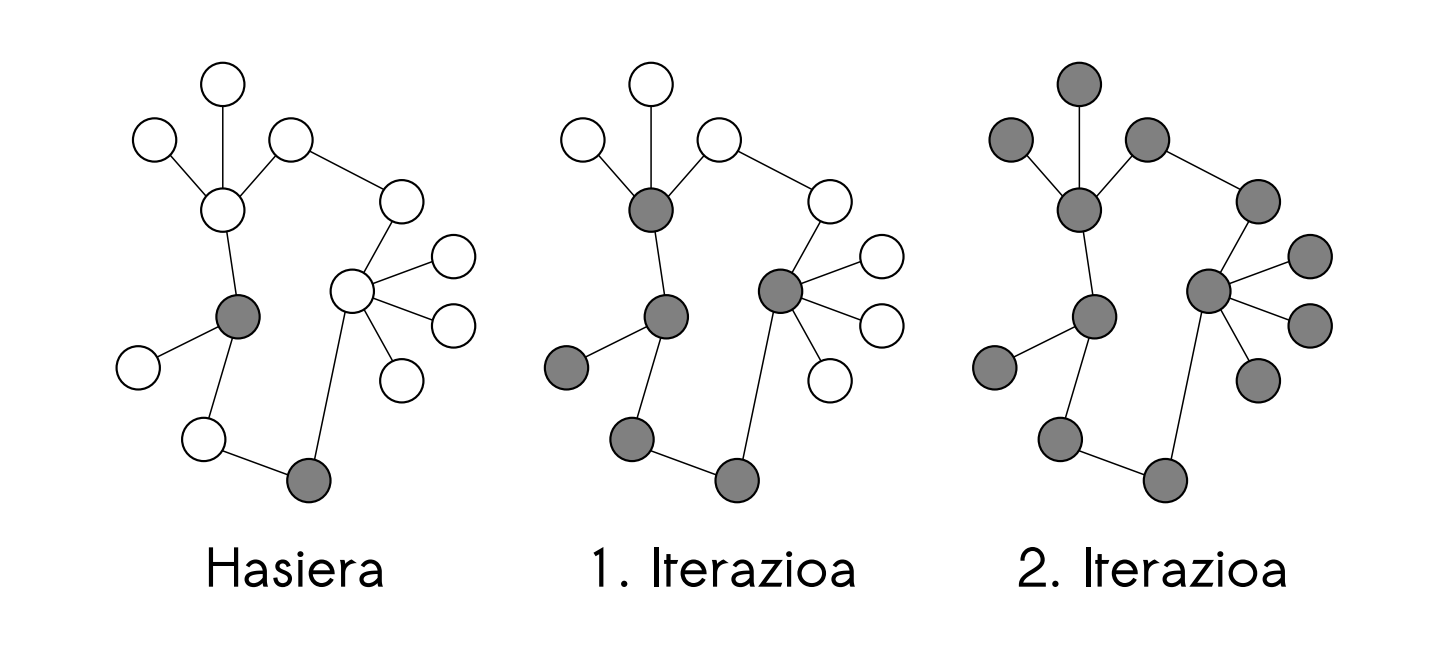
\includegraphics[scale=0.20]{adibide.png}  
 
Formaliza ezazu problema. Horretarako, definitu behar da soluzioen kodeketa, helburu funtzioaren ebaluazioa
eta, egonez gero, murrizketak. Horrez gain, soluzio onak eraikitzeko algoritmo heuristiko bat proposatu
behar da.\\

\textbf{Proiektuaren 1}. fasean problema formalizatu behar da. Horretarako, definitu behar da soluzioen kodeketa, helburu funtzioaren ebaluazioa eta, egonez gero, murrizketak. Horrez gain, soluzio onak eraikitzeko algoritmo heuristiko bat proposatu behar da.\\ 
\textbf{Proiektuaren 2}. zatian problema hau ebazteko hiru algoritmo alderatuko ditugu. Lehenengoa ausazko bilaketa bat izango da. Bigarrena, bilaketa lokala hedatzen duen algoritmo bat eta, azkenik, algoritmo memetiko bat erabiliko dugu. Hona hemen bakoitzaren azalplenak. \\
\textbf{Ausazko bilaketa.} Iterazio bakoitzean ausazko soluzio bat sortuko eta ebaluatuko da. Algoritmoaren emaitza probatu diren soluzioetatik onena izango da. \\
\textbf{Bilaketa lokalaeren hedapena}. Lehenik, problema hau bilaketa lokal baten bidez ebazteko ingurune operadore bat proposatu eta inplementatu behar da. Ondoren, operadore hori (eta beharrezkoak diren guztiak) bilaketa lokala hedatzen duen algoritmo bat sortzeko erabili beharko duzue. Hedapena edozein motakoa izan daiteke (ILS, simulated annealing, VNS, etab.). \\
\textbf{Memetikoa}. Algoritmo memetikoak genetikoak eta bilaketala lokala konbinatzen duten algoritmo hibridoak dira. Atal honetan, alde batetik, algoritmo genetiko bat aplikatzeko beharrezkoak diren operadoreak aukeratu / inplementatu behar dira. Hibridazioa egiteko, mutazio urratsean mutatzen ez diren soluzioetatik bat edo gehiago aukeratuko dira areagotzeko; hau belaunaldi guztietan edo batzuetan bakarrik egingo da. Behin hiru algoritmo hauek erabiltzeko prest, experimentazioa bi fasetan banatuko da.\\
\textbf{Parametroen egokitzapena.} Algoritmo bakoitzak dituen parametro egokiak aukeratu behar dira. Horretarako, behin parametroen balio ezberdinak probatuta, zein balioak diren egokienak argudiatuko da. \\
\textbf{Konparaketa.} Aurreko fasean aukeratutako parametroak erabiliz hiru algoritmoak konparatuko dira tamaina eta egitura ezberdineko problema instatzietan. Emaitzak aztertu eta gero, ondorioak atera beharko dituzue. \\

\pagebreak

\section{Lehenengo fasea}
\paragraph{}
Esan bezala, proiektuaren lehenengo fase honetan problemaren formalizazioa egingo dugu. Horretarako problemaren kodeketa, murrizketak, helburu funtzioa eta heuristiko pare bat azalfuko dugu.

\subsection{Soluzioen Kodeketa}
\paragraph{}
	$G \;= \;{V,E}$ grafo ez zuzendu baten aurrean gaudela suposatuko dugu. Gure soluzioa grafo honen erpinen \textit{(V)} azpimultzoa izango da, soluzioan soilik \textit{k} nodo egongo dira, eta nodo hauek soluzio bat osatuko dute:

$$S = (S_0, S_1, ... , S_k)\:, \qquad \forall i \in \lbrace 0,...,k \rbrace \quad S_i \in V$$

	Murrizketa bezala, S konbinazioa dela esan dezakegu:

$$\forall i,j( i \neq j \rightarrow S_i \neq S_j )$$

\subsection{Helburu funtzioa}
\paragraph{}

Optimizazio problema honen helburua, grafo guztian zehar komunikazioak hedatzeko behar diren pausu kopurua minimizatzean datza. Beraz, nahikoa da grafoa zeharkatzearekin soluzioak aztertzeko.\\

\fbox{\begin{minipage}{25em}
\textbf{objF} ( \textit{G} , \textit{S} )\\
 \hspace*{0.8cm} \textit{Border} $\leftarrow$ \textit{S} \\
 \hspace*{0.8cm} \textit{i} $\leftarrow$  0\\
 \hspace*{0.8cm} \textbf{While} $( \vert Border \vert > 0 )  $\\
 \hspace*{1.6cm} Set all \textit{v} $\in$ \textit{Border} as visited\\
 \hspace*{1.6cm} \textit{Border} $\leftarrow$ \textbf{expandBorder}(G, \textit{Border})\\
 \hspace*{1.6cm} \textit{i} $\leftarrow$  \textit{i} + 1\\
 \hspace*{0.8cm} \textbf{return} \textit{i} 
\end{minipage}}

\vspace*{0.5cm}

\fbox{\begin{minipage}{25em}
 \textbf{expandBorder}(G, \textit{Border})\\
  \hspace*{0.8cm} \textit{newBorder}$\leftarrow$ 0 \\
  \hspace*{0.8cm} \textbf{for all} \textit{v} $\in$ \textit{Border}\\
  \hspace*{1.6cm} \textbf{for all} $e_{vu}$ $\in$ \textit{E}\\
  \hspace*{2.4cm} \textbf{if} \textbf{not} visited \textit{u} \\
  \hspace*{3.2cm} add \textit{u} to \textit{newBorder}\\
  \hspace*{0.8cm} \textbf{return} \textit{newBorder}
\end{minipage}}

\begin{figure}[htbp]
    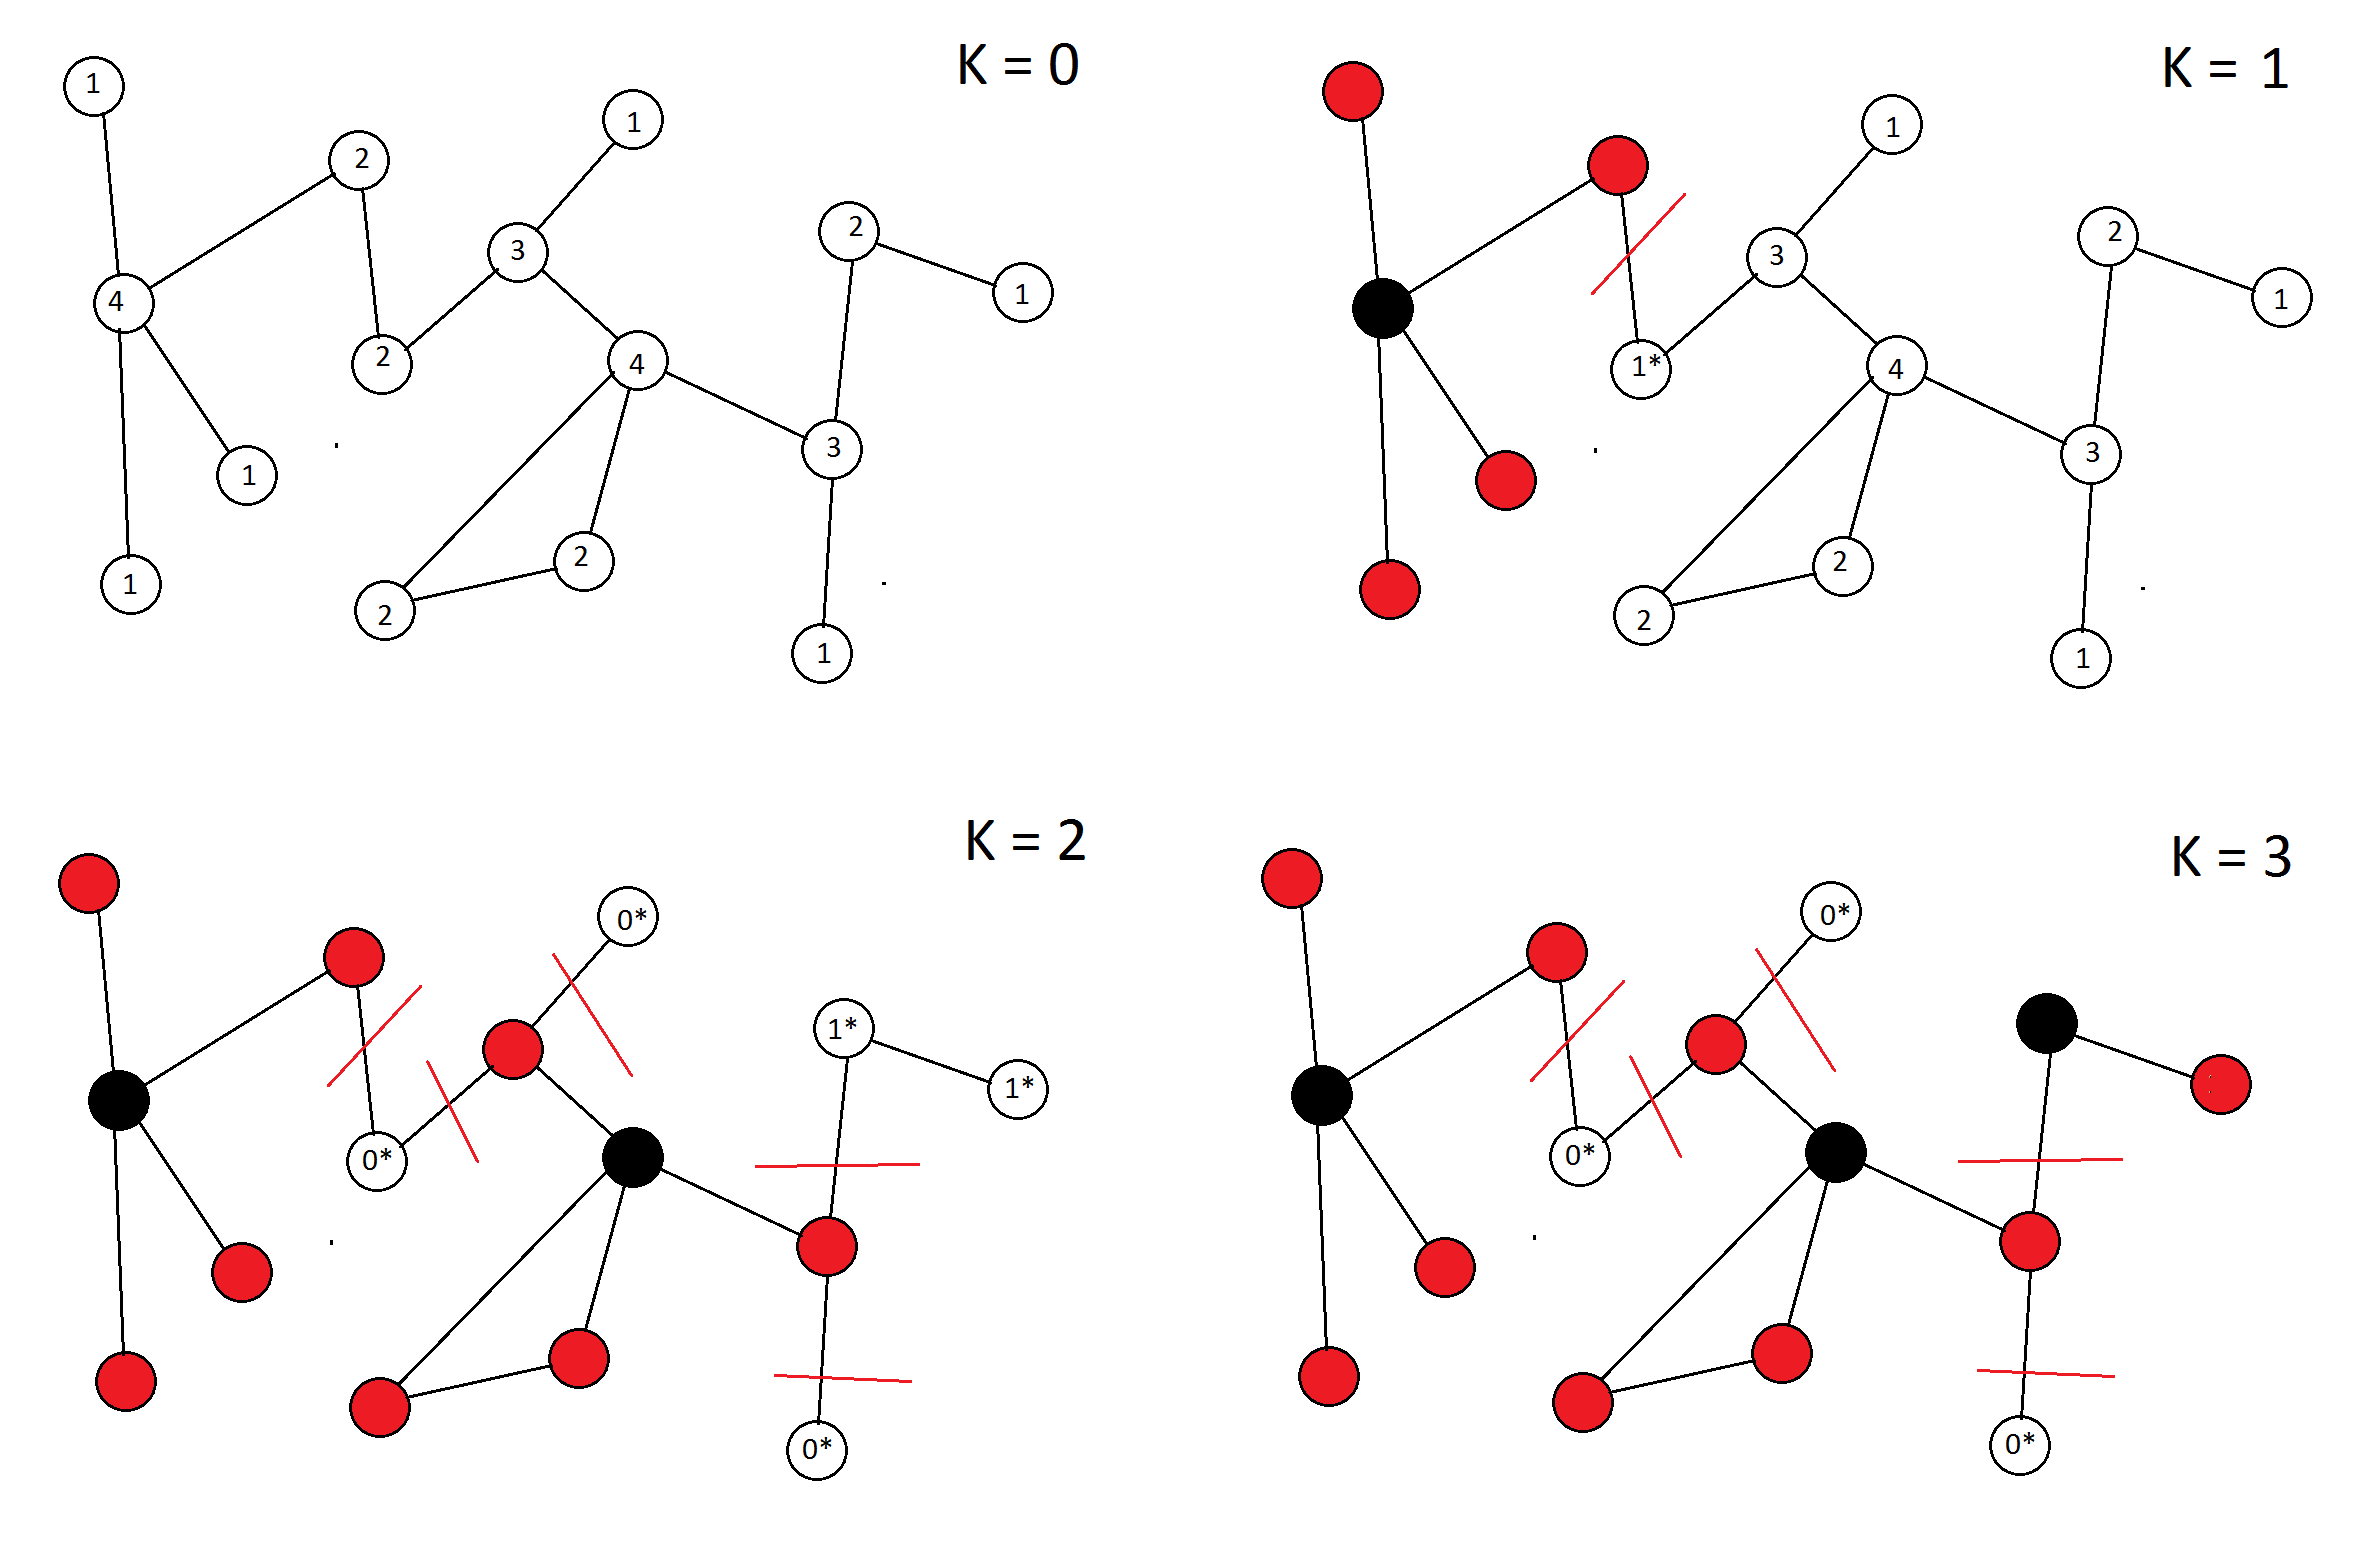
\includegraphics[scale=0.2]{Prueba0.png}
    \caption{Soluzio bilaketa heuristikoaren eta graduen eguneraketen adibidea.}
    \label{fig:adibideHeur}
\end{figure}

\subsection{Heuristikoak}
\paragraph{Lehenengo Heuristikoa}\\
Problema ebazteko soluzio eraikitzailea den algoritmo bat erabiliko dugu, hurrengo heuristikoaetan onarritzen dena.

\begin{itemize}
\item Gradu altua duten erpinek, pausu bakar batean nodo gehiago komunikatu ahal dituzte.\\

\item Auzolagun diren bi erpin hautatzea ez litzateke eraginkorra izango.
\end{itemize}

Heuristiko hau aproposa da ertz asko dituzten grafoetan aplikatzeko, grafo dentsoetan. Aitzitik, grafo ez dentsoetan(\textit{sparse}), non erpinen gradua, 2, 1 edo gehienez 3-tik igotzen ez denean, edo kate oso luzeak daudenean garrantzitsuagoa da erpin batek besteekiko duen posizioa gradua baino.

\vspace*{0.5cm}
\textbf{Algoritmoa}\\
\fbox{\begin{minipage}{30em}
 \begin{enumerate}
    \vspace*{0.3cm}
 	\item Gradurik handiena duen erpina hautatu.
 	\item Hautatutako erpina eta bere auzolagunak grafotik ezabatu.
 	\item Errepikatu 1 eta 2, \textit{k} erpin hautatu arte.
 	\vspace*{0.3cm}
 \end{enumerate}
\end{minipage}}\\
\vspace*{0.5cm}

Kontuan izatekoa da, ez duela balio graduaren arabera erpinen \textit{ranking} bat egitea. Zeren bigarren pausoan, auzolagunak ezabatzean, hauei konektatuta zeuden erpinen gradua aldatu egingo da. Hau dela eta, itzuli bakoitzean maximoa bilatu egin behar da.\\

\paragraph{Bigarren Heuristikoa}\\
	Ariketa osoan zehar kostu konputazionala alde batera utzi dudanez, heuristikoetan ere ez dut kontuan hartuko.\\
 
Distantzia eta iterazioak zuzenki proportzionalak direnez, hasiera batean pentsatu dudan heuristikoa grafo osoko urrutieneko bi nodo ekin erlazionatuta dago.\\

Behin bi urrutieneko bi nodoak izanda, beraien arteko bidea, bidea osatzen duten nodoak k multzo disjuntuetan banatuko ditugu, beti bidearen ordena errespetatuz eta bien arteko elementuen kopuru desberdintasuna minimizatuz.\\
\hspace*{2cm}	    k = 2\\
\hspace*{2cm} 		Bide luzeena:\\
\hspace*{3cm}				{a, b, c, d, e, f, g}\\
\hspace*{2cm}		k azpimultzoak:\\
\hspace*{3cm}				{a, b, c, d} eta {e, f, g}\\

K azpimultzoak izanda, multzo bakoitzaren erdian aurkitzen den nodoa aukeratuko dugu soluzioan sartzeko.\\

\hspace*{2cm}		{a, b, c, d} eta {e, f, g}\\

Heuristiko hau aplikatuta, b eta f nodoak hartuko genituzke soluzio bezala, eta grafoa solik 7 nodo hauek baditu eta zuzenean bata bestearen ondoan badaude, 2 iterazio beharko ditu mezua zabaltzeko.
Modu honetan, behin distantzia eta bidea kalkulatuta, S zuzenean izango genuke. \\

Grafoak normalean erlazio ugari dituzte, eta guzti hauek bide bakar batera txikituz zaila izango da soluzio optimora gerturatzea. Horregatik, aurreko heuristikoak grafoak zuzen baten antza dutenean egokia izango da, baino grafoari nodo eta ertz gehiago gehitzean, honen zailtasuna igoko da eta heuristikoa kaxkarragoa izango da.\\

Grafoak trinkoagoak badira, nodoen gradua ikuztea logikoagoa izango lirateke. Beraz beste heuristiko bat suposa dezakegu.\\

Honetan bide luzeena lortuko dugu ere hasieran. Baina oraingoan, bide honetako nodoen gradua kontuan izango dugu. Nodoa bidearen erdialdean dagoen heinean,  aukeratua izateko aukera gehiago izango ditu, ertzetan hurbiltzen denean plobabilitate hau txikiagotuz (ez da beharrezkoa 0-ra iristea).\\
	
\hspace*{1cm}			Bide luzeena: {a, b, c, d, e, f, g}\\
\hspace*{1cm}			Bidearen araberako probabilitateak:\\
\hspace*{2cm}				-p(a): 0'3		\hspace*{1.5cm}	-p(b): 0'4\\
\hspace*{2cm}				-p(c): 0'5		\hspace*{1.5cm}	-p(d): 0'6\\
\hspace*{2cm}				-p(e): 0'5		\hspace*{1.5cm}	-p(f): 0'4\\
\hspace*{2cm}				-p(g): 0'3\\
\hspace*{1cm}			Graduak:\\
\hspace*{2cm}				-p(a): 3 		\hspace*{1.8cm}	-p(b): 2\\
\hspace*{2cm}				-p(c): 2 		\hspace*{1.8cm}	-p(d): 3\\
\hspace*{2cm}				-p(e): 7		\hspace*{1.8cm}	-p(f): 2\\
\hspace*{2cm}				-p(g): 1\\
\hspace*{1cm}			Pisua:\\
\hspace*{2cm}		    -p(a): 0'9 		\hspace*{1.5cm}	-p(b): 0'8\\
\hspace*{2cm}			-p(c): 1 		\hspace*{1.8cm}	-p(d): 1'8\\
\hspace*{2cm}			-p(e): 3'5		\hspace*{1.5cm}	-p(f): 0'8\\
\hspace*{2cm}		    -p(g): 0'3\\

 Era honetan, nodoak gradu eta distantzia maximoko bidearen arteko pisu bat izango du (biderketa adibidez), eta hauetatik balio maximoa duen nodoa S (soluzio) multzoan sartuko dugu. Hau egin ondoren, berriro distantzia maximoa lortzen saiatuko gara, baino S-n dauden nodoak alde batera utzita, agertzen diren ertzak ere alde batera utziko ditugu.\\

\paragraph{Hirugarren Heuristikoa}
Hurrengo heuristikoa, sortzen diren subgrafoak zuhaitzak bezala tratatuko ditugu, non hautatutako erpina sustraia izango den. Beraz soluzio bat, \textit{k} zuhaitzen sustrai guztien batura izango da. Algortimoaren ideia sustraiak mugitzea da zuhaitzak orakatzeko eta hauen altuera tzikitzeko.\\

\textbf{Algoritmoa}\\
\fbox{\begin{minipage}{45em}
 \begin{enumerate}
    \vspace*{0.3cm}
 	\item Esleiturik gabeko edozein nodo hautatu
 	\item Zuhaitz bat sortu nodo horretatik, $\frac{V}{k} $ tamainakoa gutzi gora-behera.
 	\item Errepikatu pausu hauek \textit{V}-ko nodo guztiak hartu arte eta \textit{k} zuhaitz izan arte.
 	\item Zuhaitz bakoitzean sakonera bilaketa bat egin eta aurkitu sustraitik ateratzen diren bi adar luzeenak.
 	\item Bi bide hauen arabera sustraiaren posizio berria kalkulatu. (Adibidean ikusten den moduan, bide luzeari laburra gehitu, 6 distantziako bide bat izango dugu, non 3. nodoa erdia da, $\frac{6}{2} = 3 , \quad 3 - 2 = 1$, pausu bat bide luzea duen adarretik mugitu behar gara). 
 	\vspace*{0.3cm}
 \end{enumerate}
\end{minipage}}
\vspace*{0.5cm}

Algoritmoaren azken atal honetan bilaketa lokala bilaketa lokala ere egin daiteke, zuhaitzaren altuera minimizatzeko helburu funtzioa definituz, baina komputazionalki askoz garestiagoa izango dela dirudi.

\begin{figure}[htbp]
    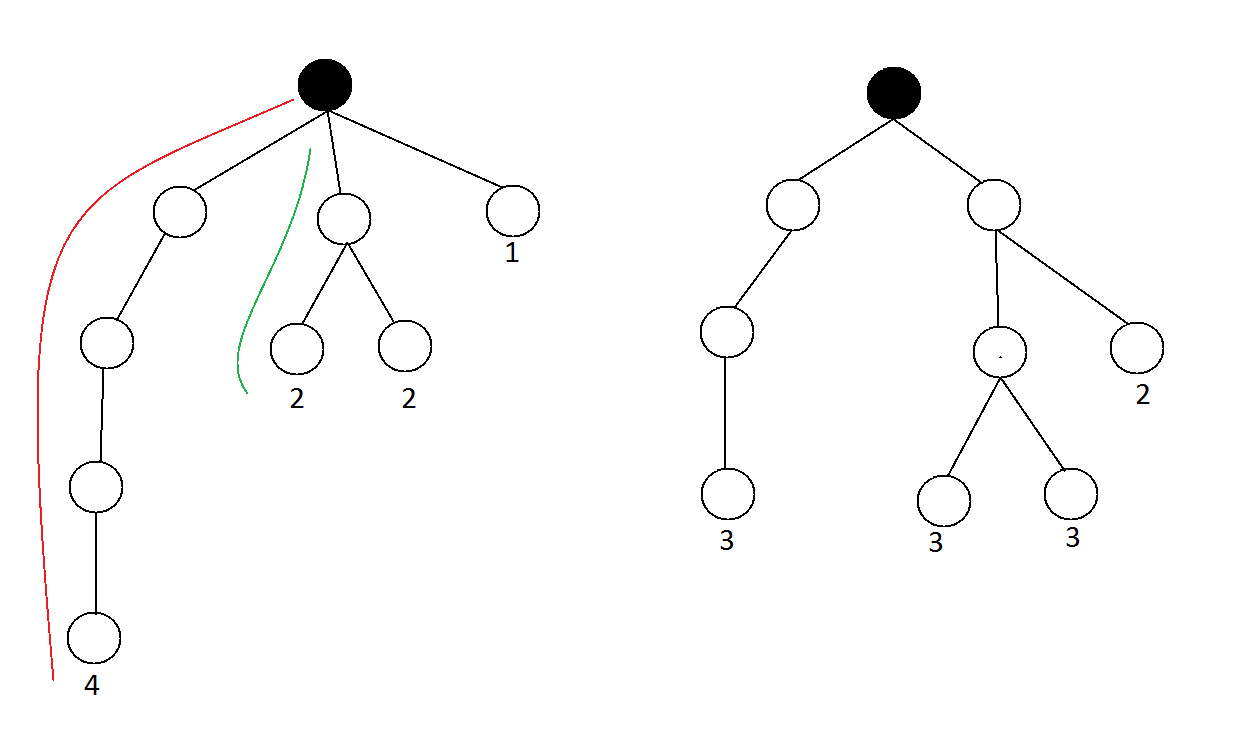
\includegraphics[scale=0.3]{pruebaArbol.png}
    \caption{Zuhaitz orekatze adibidea.}
    \label{fig:adibideHeur}
\end{figure}

\pagebreak
\section{Bigarren fasea}
\paragraph{}
	Behin gure problema formalizatua dugula, problema bera burutzeko erabiliko diren algoritmoak azalduko ditugu. Behin algoritmoak azalduta, hauen esperimentazioa egingo dugu, bertan parametroen egokitzapena azalduko dugu, baita algoritmoen konparaketa azkar bat egingo da. Behin datu guztiak jasota izanda ondorio zuzen bat lortu ahal izateko.


\subsection{Algoritmoen azalpena}
\paragraph{}
	Atal honetan proiektua garatzeko sortu ditugun algoritmo desberdinen azalpen bat egingo dugu, horretarako banan banan analizitatuko ditugu.

\subsubsection{GraphComunicationProblem}
\paragraph{}
	Funtzio honek grafo bat jasota, honekin egin daitezkeen funtzio desberdinak sortuko ditu, evaluate, debug, valid, correct eta saveSnapshop.

\subsubsection{Evaluate} 
\paragraph{}
	  Funtzio honi soluzio bat besterik ez zaio pasa behar. \textit{GraphComunicationProblem.R} fitxategiaren barruan aurkitzen da, beraz grafoa zuzenean atzigarri izango du, eta honen beharrik ez du izango sarrera parametroetan.\\

	Funtzioa modu eraginkor batean egitea beharrezkoa zela ikusi genuen, azken finean behin eta berriro gehien errepikatuko den funtzioa da. Harierako fasean proposatu genuen funtzioa aldatu egin dugu, erpinen propietate bat aurki genuenean. Orain, hiru bektore nagusi izango ditugu momentu horo: border, oldborder eta new border.\\
	
\begin{itemize}
\item[•]\textit{Border}: Iterazio honetan analizatuko diren erpinen multzoa da.(Inizialki soluzioa)
\item[•]\textit{Old border}: Aurreko iterazioan \textit{Border}-en egondako erpinak. 
\item[•]\textit{New border}: Hurrengo iterazioan \textit{Border}-en egongo diren erpinak. 
\end{itemize}

Beraz, une oro, hiru ertz mota dauzkate Borderren dauden erpinek, Old borderrera doazenak, \textit{Border}-era doazenak eta \textit{New Border}-era doazenak, aurreko biak kenduta, New border izango dugu. Soluzio honen abaintaia, gure iritziz, erpin bakoitza behin bakarrik igaroko da Border, Old border eta New borderretik, baita ere erpin multzo hauetan egiten diren eragiketak errazten ez dutelako grafo osoa erabiltzen baizik eta zati txiki bat.\\

Hurrengo irudian ikusi daiteke kolorez gorriz komunikatu gabeko erpinak eta urdinez komunikatutakoak, algoritmoa ez da berriro hauetatik igaroko. Horiz dauden erpinak Borderri dagozkio, berdez Old borderri dagozkionak.

\begin{table}[hbt!]
\centering
\begin{tabular}{c c c}
\begin{center}
    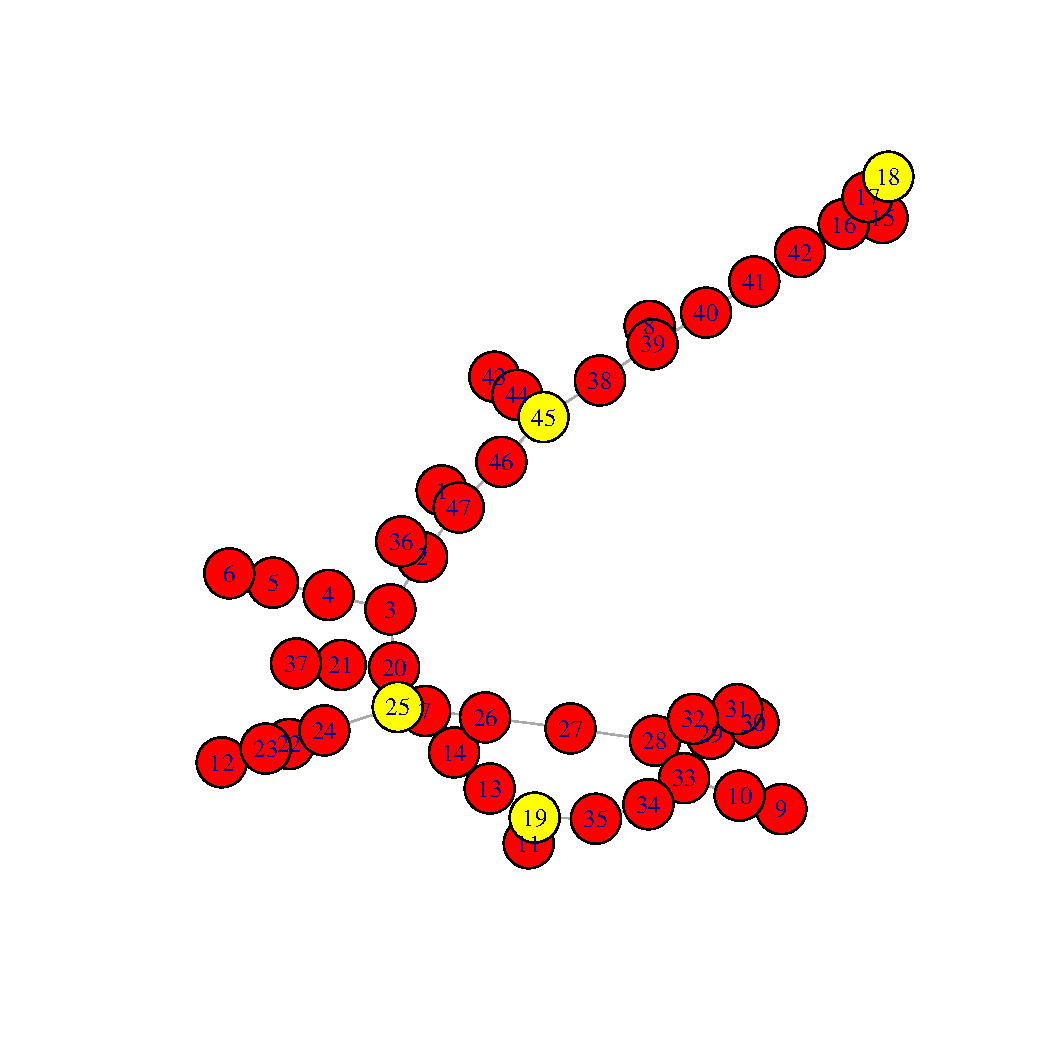
\includegraphics[scale=0.3]{graph0.pdf}
\end{center}
&
\begin{center}
    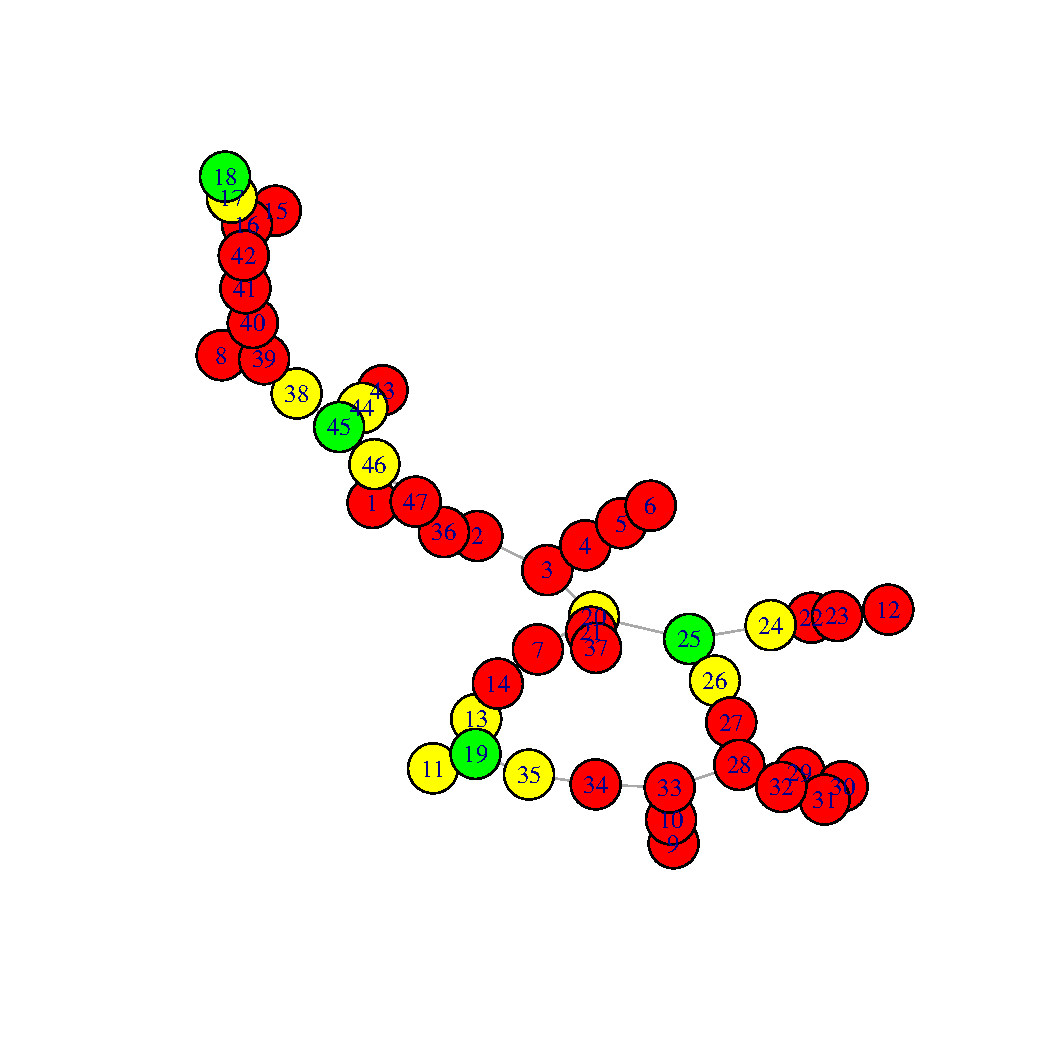
\includegraphics[scale=0.3]{graph1.pdf}
\end{center}
&
\begin{center}
    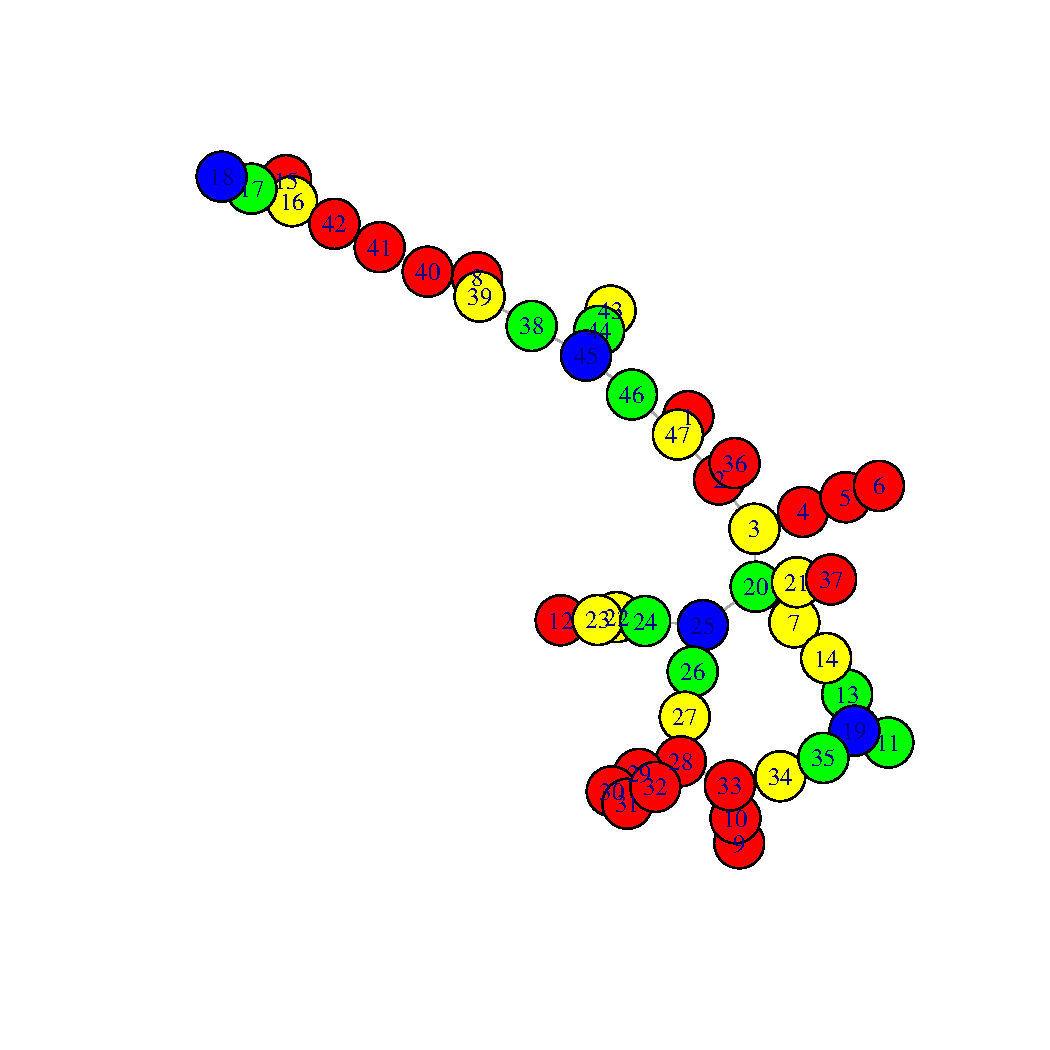
\includegraphics[scale=0.3]{graph2.pdf}
\end{center}\\

\begin{center}
    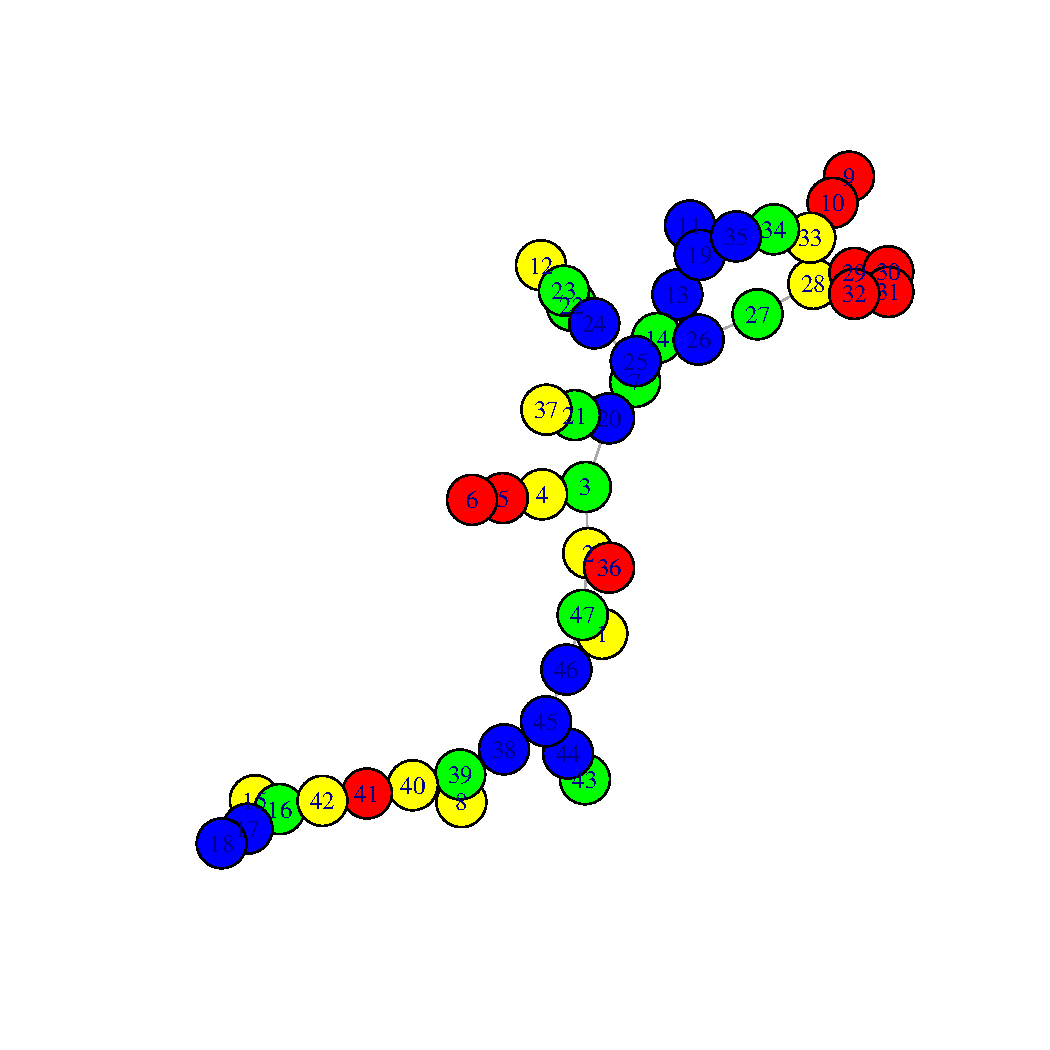
\includegraphics[scale=0.3]{graph3.pdf}
\end{center}
&
\begin{center}
    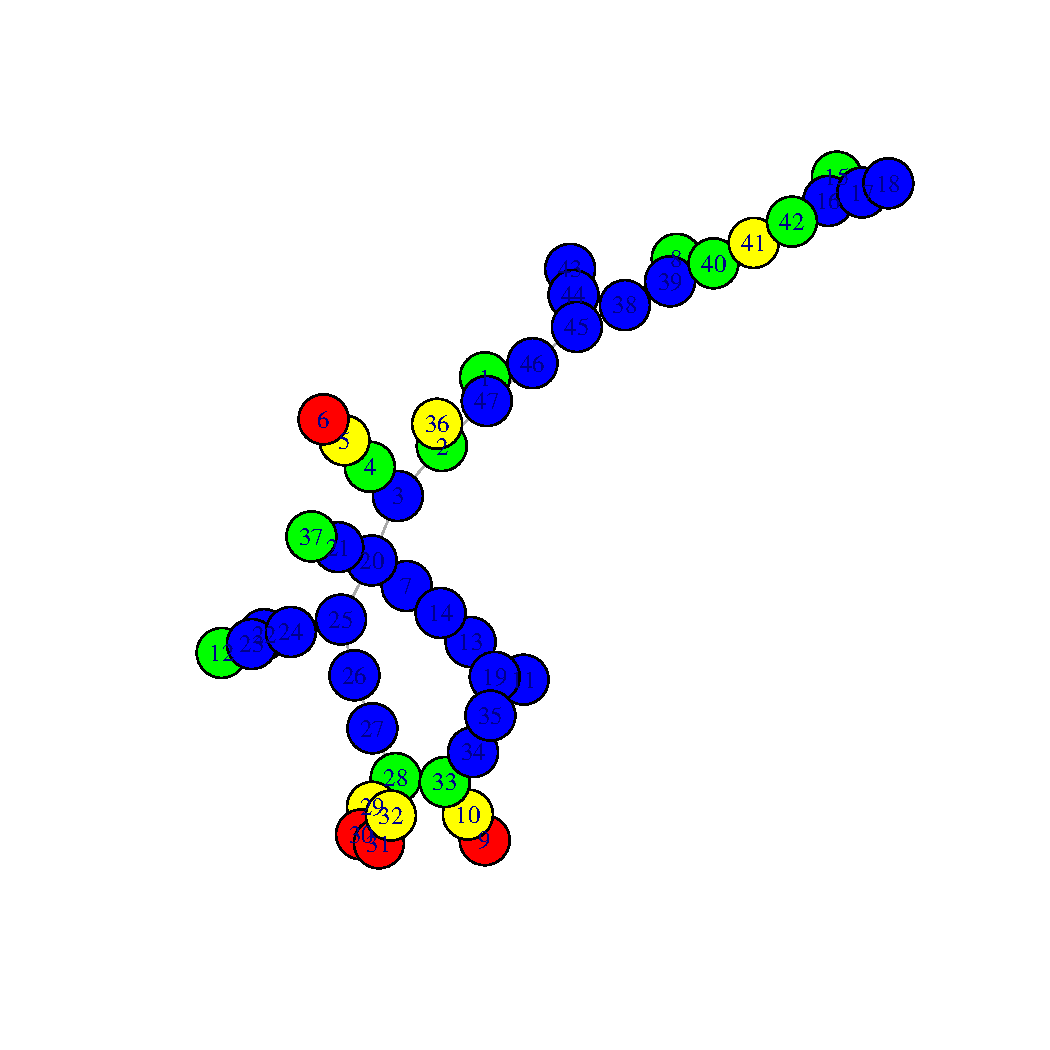
\includegraphics[scale=0.3]{graph4.pdf}
\end{center}
&
\begin{center}
    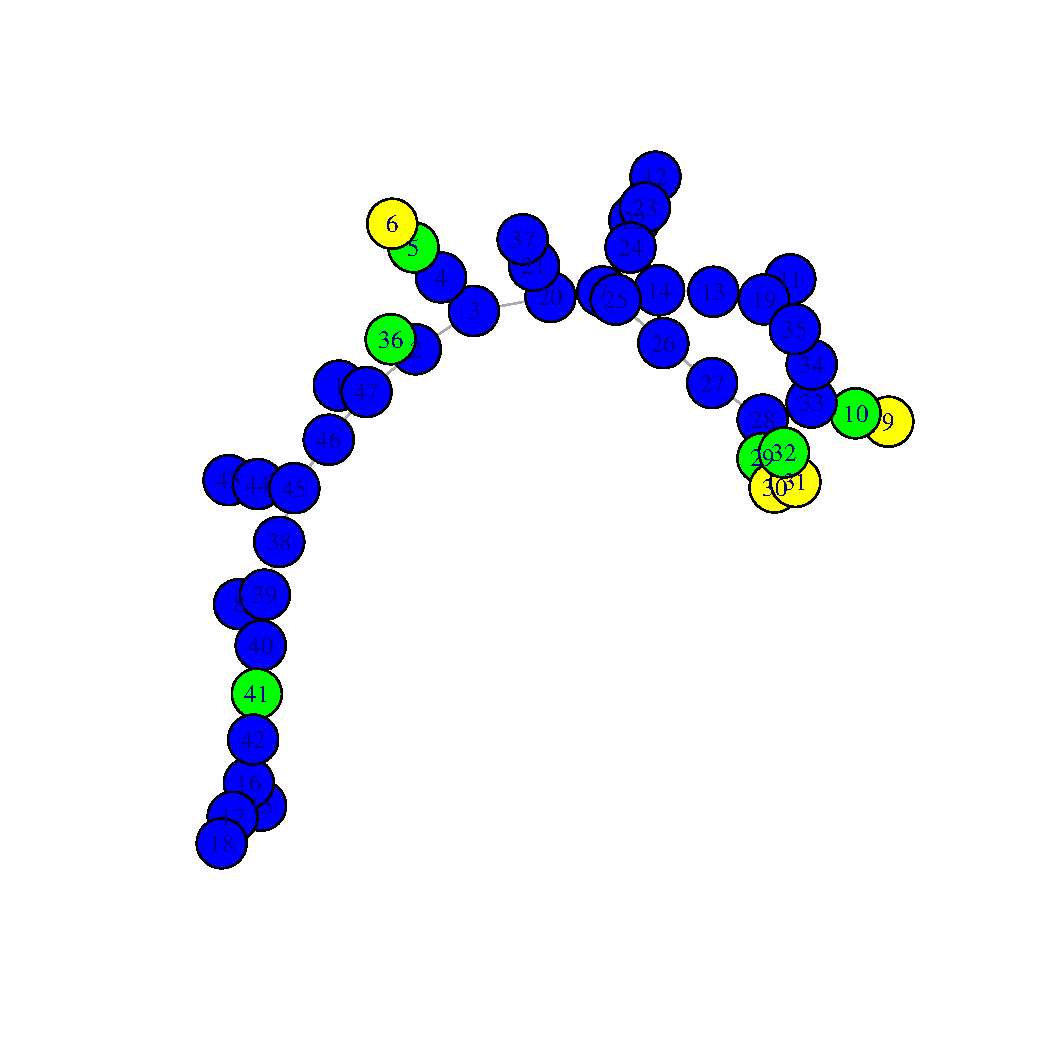
\includegraphics[scale=0.3]{graph5.pdf}
\end{center}
\\
\end{tabular}
\caption{Evaluazio funtzioaren portaera grafikoki erakutsita.}
\end{table}

\subsubsection{Valid}
\paragraph{}
	Soluzio bat egokia den edo ez jakiteko funtzio bat egitea egokia dela ikusi dugu. Funtzio honek soluzio bat emanda, honek murriztapenak betetzen dituen adieraziko digu, True edo False itzuliz. True murriztapenak betetzen baditu eta False hauekez baditu betetzen.\\
	Murriztapenak hauek dira:
	\begin{itemize}
	
\item[•]Soluzioaren luzeera ezin du grafoaren nodo kopurua gainditu, ezta 1 baino txikiagoa izan. 
\item[•]Soluzioa ezin ditu balio errepikaturik izan ez balio hutsik.
\item[•]Soluzioaren baliak, 1 eta nodo kopuruaren artekoa izan behar du.
\end{itemize}

\subsubsection{Debug}
\paragraph{}
	Evaluate funtzioa sortzeko, debug bat erabili genuen, eta honen laguntza oso egokia dela ikusita, guztiz ezabatu ordez kontzerbatu egin dugu.\\
	
Soluzio bat emanda funtzio honek border, newboerder eta oldborder multzoen nodoak printatzen ditu kolore desberdinetan grafoan iterazioz iterazio. Irudietan ikusten denbezala.\\

\subsubsection{saveSnapshop}
\paragraph{}
	Debug funtzioa printatzeko erabiltzen duen funtzioa da. \\
Grafoa, dokumentu baten izena eta kolore desberinak emanez, grafoko nodoak koloreztatuko ditu. \\

\subsubsection{localSearch}
\paragraph{}
	Bilaketa lokala egiteko, Metaheur paketeko bilaketak erabiltzea pentsatu dugu. Horretarako neigborhood bat implementatu behar izan dugu, \textit{insertNeigborhood}. Bertan, \textit{setValidity}, \textit{nextNeighbor}, \textit{hasMoreNeighbors}, \textit{resetNeighborhood} eta \textit{insertNeighborhood} funtzioak berraldatu ditugu nuk nahi dugun ingurunea definitzeko.\\ 
	
	Gure ingurunea soluzioaren zenbaki bat bat goruntz edo beruntz aldatzea da, beti ahal bada ere. Zenbakia 1 bada, N bada edo soluzioko beste zenbaki baten diferentzia 1 bada, balioak errepikatu ahalko ez diren konbinaketak sortuko dira, baita zenbaki bat 0 edo N+1 izango ez diren soluzioak.\\
	
	Aurreko ingurunea txikia dela ikusita, eskuz beste bi ingurune programatu ditugu, +2 eta  -2 ingurunea eta +1, +2, -1 eta -2 inguruneak. Hau da, dagoen zenbakiari 1 edo 2 gehituta edo kenduta lortuko ziren emaitzak. 
	Ingurunearen Random aukera ez dugu erabiltzen, hau da, beti ordenean exekutatuko dira ingurune guztiak.\\

\subsubsection{randomSearch}
\paragraph{}
	Auzazko bilaketa burutzeko, k luzeerako auzaz aukeratutako 1-etik n-rako zenbakiaz sortuta dagoen 10 soluzio sortzen dira, hauetatik eval funtzioa aplikatuta emaitza hoberena duen soluzioa itzuliko da. 

\subsubsection{Memetic Algorithm}
\paragraph{}
	Lehendabizi, algoritmo genetikoa, erabilitako kodeketarako egokitzeko, gurutzaketa (\textit{cross}) eta mutaketa funtzioak sortu ditugu. Lehenengoa, bi soluzio izanda, hauen diferentzia bakarrik gurutzatuko da, diferentzia bitan banatu behar da, gen guztiak aldatzen baidira, hasierako soluzio berdinak izango genituzke, hemen biderkaketa beti beherantz borobiltzea erabaki dugu. Aldatuko diren gene kopurua izanda, auzas aukeratuko dira eskuragarri daudenen artean. Beztalde, mutaketa funtzioa, askoz simpleagoa da eta auzaz aukeratutako soluzioaren gen bat aldatzen beste edosein gen bategatik, soluzio bideragarri bat izan arte.\\
	
	Honekin, algoritmo genetikoa gure probleman erabiltzeko prest zegoen, mememitikoa egiteko, \textit{metaHeur} paketean zegoen \textit{basicGenetikAlgorithm} funtzioa aldatu egin dugu, berezi mutazioak egin eta gero, mutatzen ez diren soluzioak bilaketa lokal bat egiteko aukera berdina izango dute, parametro bezala izango dira ingurunea eta soluzio hautatzailea, berez \textit{metaHeur} paketean dagoen \textit{LocalSearch} algoritmoa erabiltzen da bilaketa lokalerako eta \textit{FirstImprovementSelector} soluzio hautatzaile bezala. Erabilitako ingurunea, 2.1.6 atalean aipatutakoa da.\\

\pagebreak
\section{Esperimentazioa}
\paragraph{}
Algoritmoak sortuta daudela, hauek probatzea eta konparatzea baino ez da geratzen. Horretarako, erabiliko ditugun grafoak sortu beharko ditugu modu eta tamaina desberdinetan. Grafoak izan eta gero algoritmoak exekutatzea baino ez da faltako.
 
\subsection{Grafo instantzien deskribapena}
\paragraph{}
Probak egiteko, hiru grafo desberdin sortzea egokia izango litzakeela iruditu zitzaigun. Hiru grafo mota erabiltzeaz gain, bakoitzerako bi tamaina desberdin ere ezberdindu ditugu; txikiak eta handiak, 50 eta 200 erpin ingurukoak.\\

Gure probleman, konektibitatearen murrizpena dela eta, grafoa sortu ondoren multzo konexu handiena hartzen dugu.\\

\begin{itemize}
\item[•]\textbf{Erdos Renyi Game} ausazko grafo bat sortzeko erabiltzen diren bi eredu aurkezten ditu, G(n,m) eta G(n,p) . G(n,p) ereduan, gafoko n erpinak auzaz konektatzen dira. Erpin bakoitza p probabilitatearekin aukeratzen da. Bi ereduetan, n erpin eta m ertz dituzten grafo guztiek probabilitate berdina dute.
\item[•]\textbf{Aging Ba Game}Funtzio honek grafoaren eboluzioaren simulazioaren bitartez sortzen ditu auzazko grafoak. Erpin berri bat sortzen den bakoitzean, sortuta dagoen erpin batera lotuko da, eta aukeratzen den erpina, erpinaren adinaren eta graduaren araberako probabilitate batez aukeratuko da.\\Gure proiektua sare sozial baten inguruan dagoenez, grafo egokienak modu honetara sotuko direla uste dugu. 
\item[•]\textbf{Watts Strogatz Game} Lehendabizi erpin guztiak sortzen dira, eta gero hauen gainean ertzak, p probabilitate bat izanda. Kontuan eduki beharko da grafoak sortzeko modu honek ertz errepikatuak eta bukleak sor ditzazke.\\
\end{itemize}


\subsection{K parametroen egokitzapena}
\paragraph{}
Grafo tamaina bakoitzerako k desberdin bat sortu dugu, txikientzat 5 eta handienentzat 7.\\

K eta n araberakoa izango da soluzio posible kopurua. K = n bada soluzio bakarra izango dugu, eta K txikiagoa bada soluzio posible gehiegi eta k txikiegia bada soluzio posible gutxiegi, beraz bi tamainentzako k desberdinak definitzea pentsatu dugu. Arazo berdinean soluzio posible desberdinak izateko, modu honetan grafo txikiak 2,11e6 eta handiak 4,4e14 soluzio posible izango dituzte hain zuzen ere.\\

\subsection{Errekutsoak}
\paragraph{}
Esperimentazioa egiteko algoritmo guztiak denbora berdina grafiko berean exekutatzea pentsatu dugu, hauek denboran zehar duten eboluzioa ikusi ahal izateko. Hau da, auzazko bilaketa, bilaketa lokala eta memetikoa denbora bera exekutatuko dugu lortutako emaitzak komparatu ahal izateko.\\
 
K bezala, grafo txikienak 60 segundo exekutatuko dira, eta handiak 80 segundu. 

\pagebreak
\subsection{Grafo mota desberdinak eta ingurune desberdinak \textit{LocalSearch} arabera}
\paragraph{}
	Esan bezala, 6 grafo multzo ditugu, baina multzo bakoitzerako hiru ingurune exekutatu ditugu, aldaketak ikusteko. Lehen eta bigarren inguruneak oso antzekoak dira (bat gora/bera edo bi gora/bera),  baina hirugarrena bien arteko konbinazioa dela esan dezakegu, beraz, besteak baino handiagoa dela ikusiko dugu eta honek duen ondoria somatzea espero dugu.  Era berean, grafo desberdinen aurrean gure algoritmoa duen joera ere ikusi beharko genuke.\\
	
Ebaluaketa kopurua murrizketen araberakoa da, eta hauek handitu eta txikitu daitzezke hasierako soluzioaren arabera.\\


\begin{center}	
\begin{knitrout}
\definecolor{shadecolor}{rgb}{0.969, 0.969, 0.969}\color{fgcolor}\begin{figure}[!h]
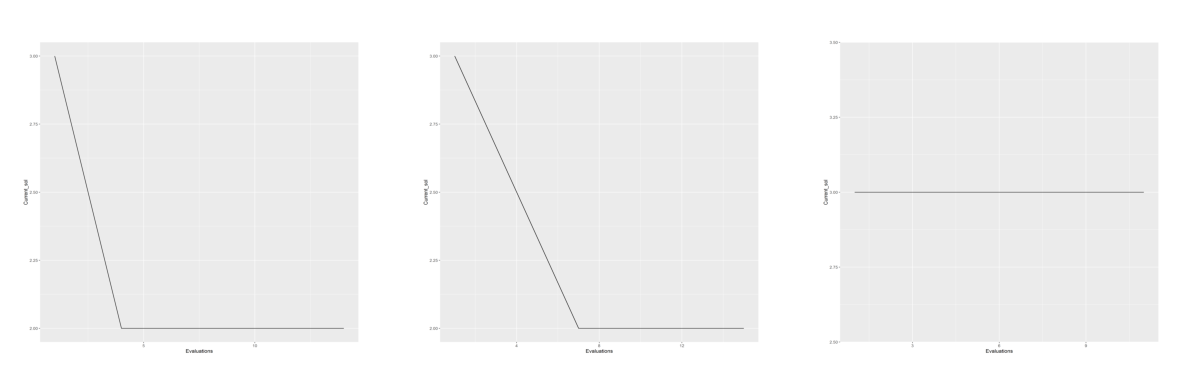
\includegraphics[width=\maxwidth]{figure/unnamed-chunk-1-1} \caption[Grafo txikiak, Aging motakoak, lehen ingurunea erabilita]{Grafo txikiak, Aging motakoak, lehen ingurunea erabilita}\label{fig:unnamed-chunk-1}
\end{figure}


\end{knitrout}
\end{center}

\begin{center}	
\begin{knitrout}
\definecolor{shadecolor}{rgb}{0.969, 0.969, 0.969}\color{fgcolor}\begin{figure}[!h]
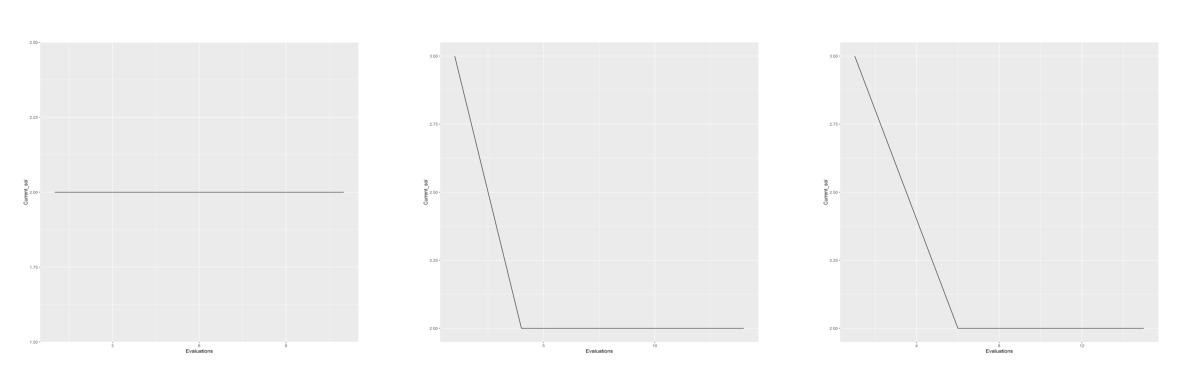
\includegraphics[width=\maxwidth]{figure/unnamed-chunk-2-1} \caption[Grafo txikiak, Aging motakoak, bigarren ingurunea erabilita]{Grafo txikiak, Aging motakoak, bigarren ingurunea erabilita}\label{fig:unnamed-chunk-2}
\end{figure}


\end{knitrout}
\end{center}

\pagebreak
\begin{center}	
\begin{knitrout}
\definecolor{shadecolor}{rgb}{0.969, 0.969, 0.969}\color{fgcolor}\begin{figure}[!h]
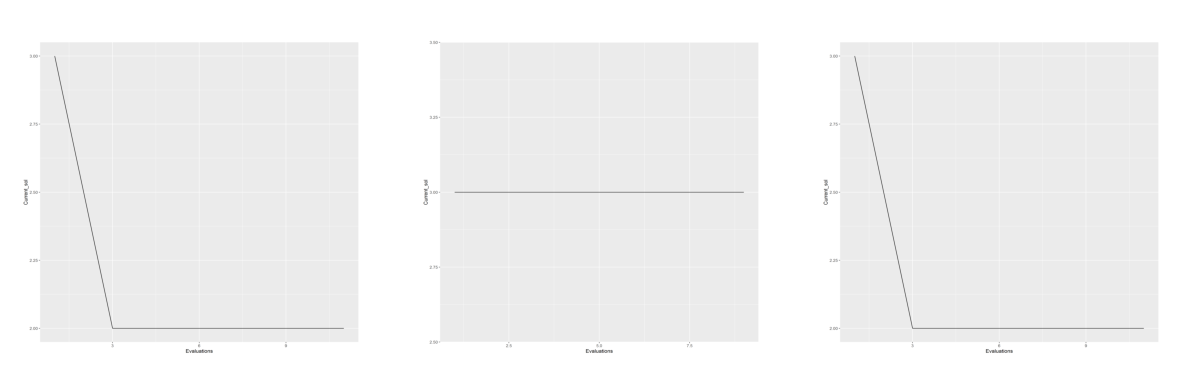
\includegraphics[width=\maxwidth]{figure/unnamed-chunk-3-1} \caption[Grafo txikiak, Aging motakoak, hirugarren ingurunea erabilita]{Grafo txikiak, Aging motakoak, hirugarren ingurunea erabilita}\label{fig:unnamed-chunk-3}
\end{figure}


\end{knitrout}
\end{center}

Grafoetan ikusi daiteke emaitza optimoa 2 dela beti eta beti lortu da, lehengo ingurunea erabilita hirugarren grafoan izan ezik, baina orokorrean 2 lortzea ez da zaila. Ikusten dugun bezala, zuzenean edo pauso bakar batean lortuko dugu 2 balio duen emaitza, eta zuzenean ez bada, lehenengoan 3 topatuko dugu beti.\\

\begin{center}	
\begin{knitrout}
\definecolor{shadecolor}{rgb}{0.969, 0.969, 0.969}\color{fgcolor}\begin{figure}[!h]
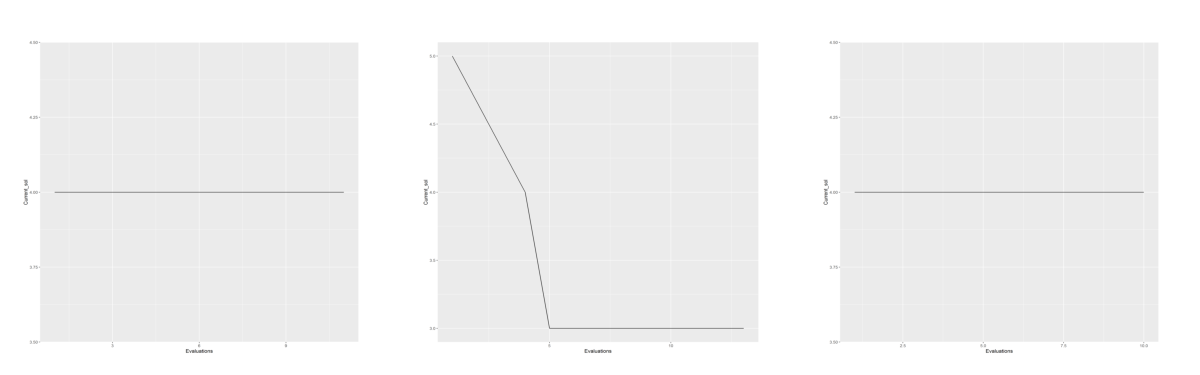
\includegraphics[width=\maxwidth]{figure/unnamed-chunk-4-1} \caption[Grafo txikiak, Erdos motakoak, lehen ingurunea erabilita]{Grafo txikiak, Erdos motakoak, lehen ingurunea erabilita}\label{fig:unnamed-chunk-4}
\end{figure}


\end{knitrout}
\end{center}

\begin{center}	
\begin{knitrout}
\definecolor{shadecolor}{rgb}{0.969, 0.969, 0.969}\color{fgcolor}\begin{figure}[!h]
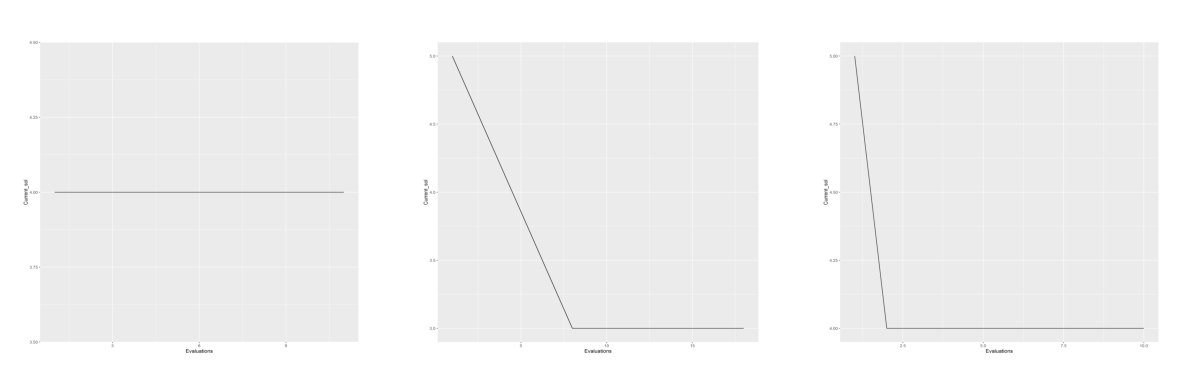
\includegraphics[width=\maxwidth]{figure/unnamed-chunk-5-1} \caption[Grafo txikiak, Erdos motakoak, bigarren ingurunea erabilita]{Grafo txikiak, Erdos motakoak, bigarren ingurunea erabilita}\label{fig:unnamed-chunk-5}
\end{figure}


\end{knitrout}
\end{center}

\begin{center}	
\begin{knitrout}
\definecolor{shadecolor}{rgb}{0.969, 0.969, 0.969}\color{fgcolor}\begin{figure}[!h]
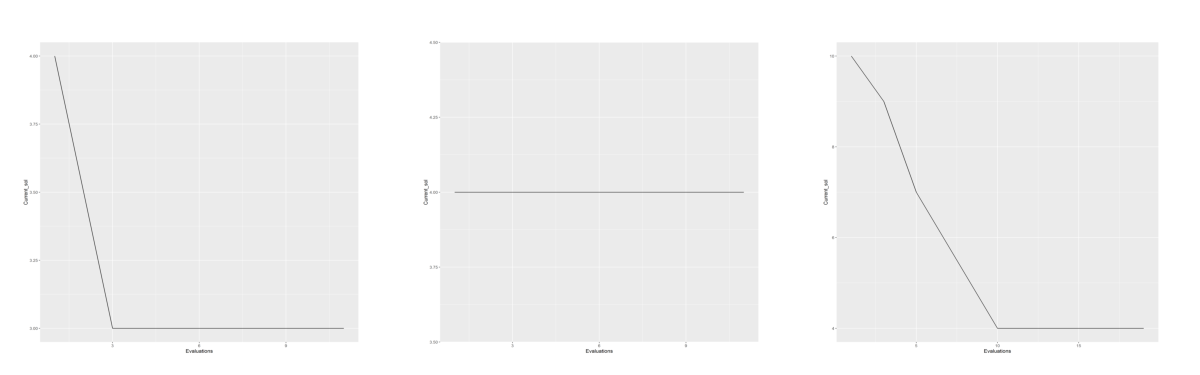
\includegraphics[width=\maxwidth]{figure/unnamed-chunk-6-1} \caption[Grafo txikiak, Erdos motakoak, hirugarren ingurunea erabilita]{Grafo txikiak, Erdos motakoak, hirugarren ingurunea erabilita}\label{fig:unnamed-chunk-6}
\end{figure}


\end{knitrout}
\end{center}
\pagebreak
Emaitza optimoa 3 dela ikus daiteke honen arabera (exekutatuetatik optimoa 3 delako), beti ez lortu harren. Baina horaingo hauetan, LocalSearch algoritmoak pauso bat baino gehiago behar izan ditu optimoa lortzeko. Azkenekoan ikusi daiteke hiru aldiz aldatu duela soluzioa optimoa topatu arte.\\

	Lehenengo soluzio bezala ere balio desberdinak topa daitezke, hau da, ez da beti hiru izango agign grafoetan bezela. Adibidez azkeneko grafikoan 10etik 9ra eta 9tik 7ra pasatuko da azkenik 7tik 4ra iristeko. Hemen ingurunea banan banan ez duela zertan obetu behar ikus dezakegu eta optimoa lortzeko aukerak gutxiago direla ere, ala ere, exekutatutako denboran (60segundu) ingurune guztiak hiru topatu dute optimotzat.\\
	
\begin{center}	
\begin{knitrout}
\definecolor{shadecolor}{rgb}{0.969, 0.969, 0.969}\color{fgcolor}\begin{figure}[!h]
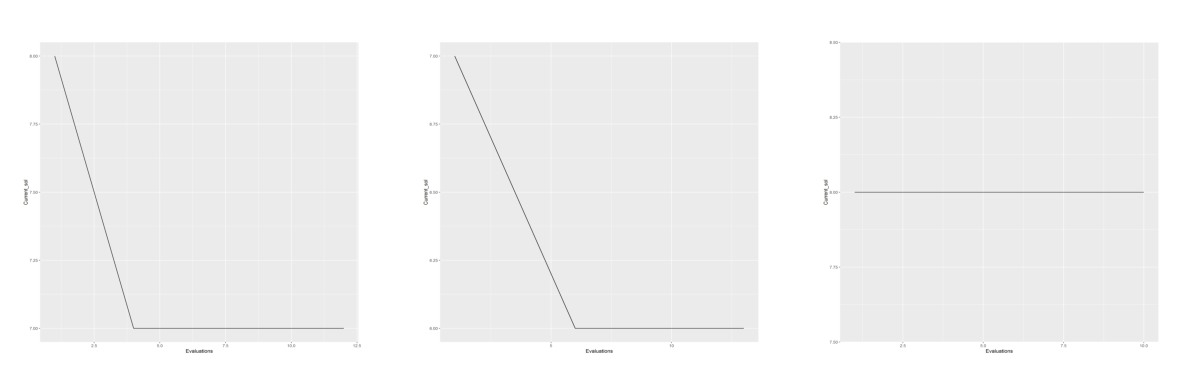
\includegraphics[width=\maxwidth]{figure/unnamed-chunk-7-1} \caption[Grafo txikiak, Watts motakoak, lehen ingurunea erabilita]{Grafo txikiak, Watts motakoak, lehen ingurunea erabilita}\label{fig:unnamed-chunk-7}
\end{figure}


\end{knitrout}
\end{center}

\begin{center}	
\begin{knitrout}
\definecolor{shadecolor}{rgb}{0.969, 0.969, 0.969}\color{fgcolor}\begin{figure}[!h]
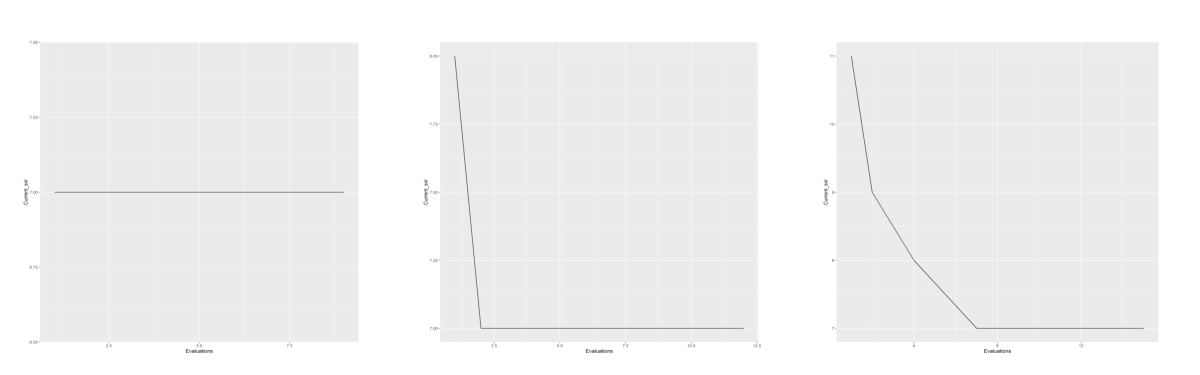
\includegraphics[width=\maxwidth]{figure/unnamed-chunk-8-1} \caption[Grafo txikiak, Watts motakoak, bigarren ingurunea erabilita]{Grafo txikiak, Watts motakoak, bigarren ingurunea erabilita}\label{fig:unnamed-chunk-8}
\end{figure}


\end{knitrout}
\end{center}

\begin{center}	
\begin{knitrout}
\definecolor{shadecolor}{rgb}{0.969, 0.969, 0.969}\color{fgcolor}\begin{figure}[!h]
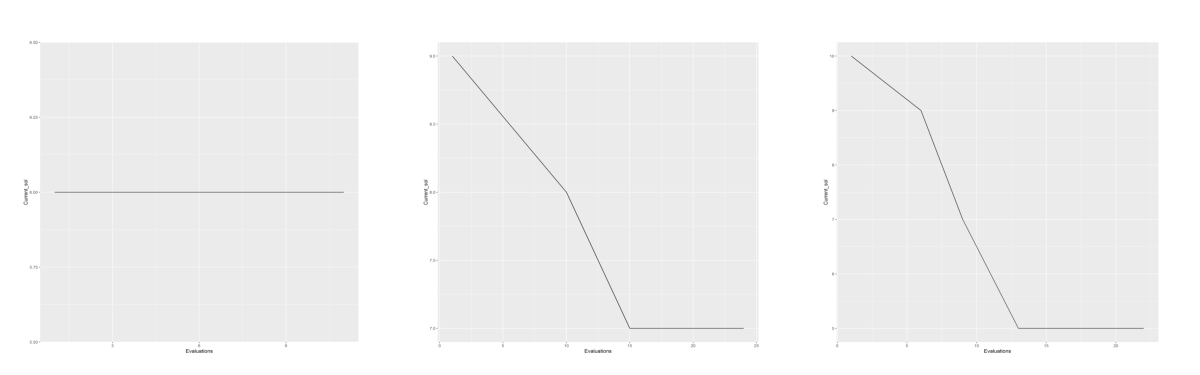
\includegraphics[width=\maxwidth]{figure/unnamed-chunk-9-1} \caption[Grafo txikiak, Watts motakoak, hirugarren ingurunea erabilita]{Grafo txikiak, Watts motakoak, hirugarren ingurunea erabilita}\label{fig:unnamed-chunk-9}
\end{figure}


\end{knitrout}
\end{center}
\vspace*{0.1cm}
Kasu honetan, emaitza desberdinak topatzen ditugu, 8-tik 5-era, lehenengo ingurunea eta bigarren ingurunea erabilita 8 eta 7 lortuko dugu gehienetan, baina hirugarren ingurunea erabilita, hiru pausotan 5 lortu dugula ikusi dezakegu.\\

\begin{center}	
\begin{knitrout}
\definecolor{shadecolor}{rgb}{0.969, 0.969, 0.969}\color{fgcolor}\begin{figure}[!h]
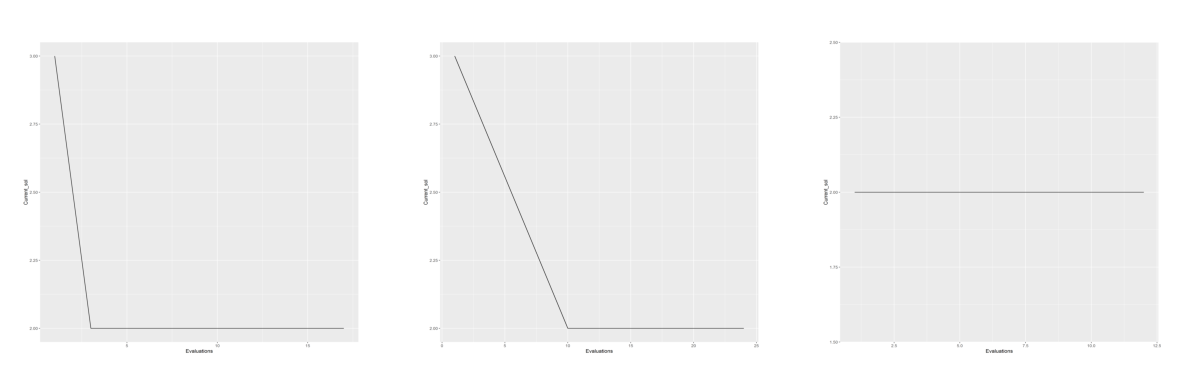
\includegraphics[width=\maxwidth]{figure/unnamed-chunk-10-1} \caption[Grafo handiak, Erdos motakoak, lehen ingurunea erabilita]{Grafo handiak, Erdos motakoak, lehen ingurunea erabilita}\label{fig:unnamed-chunk-10}
\end{figure}


\end{knitrout}
\end{center}

\begin{center}	
\begin{knitrout}
\definecolor{shadecolor}{rgb}{0.969, 0.969, 0.969}\color{fgcolor}\begin{figure}[!h]
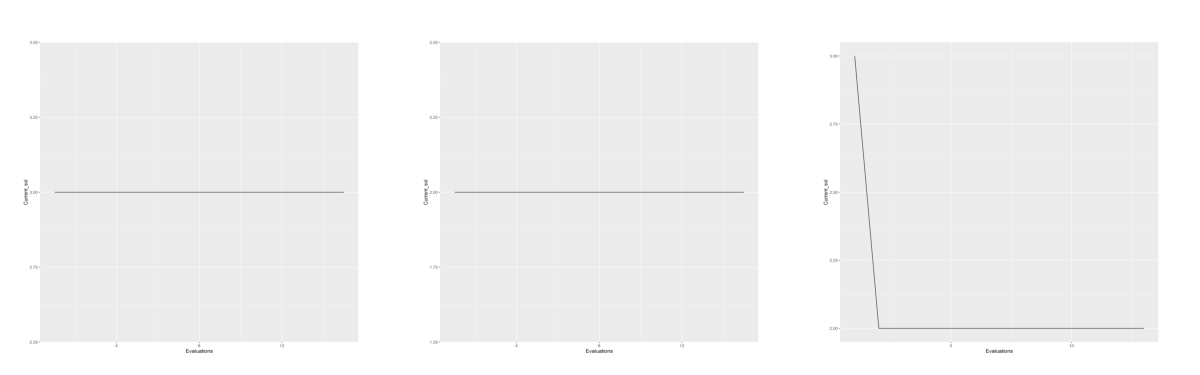
\includegraphics[width=\maxwidth]{figure/unnamed-chunk-11-1} \caption[Grafo handiak, Erdos motakoak, bigarren ingurunea erabilita]{Grafo handiak, Erdos motakoak, bigarren ingurunea erabilita}\label{fig:unnamed-chunk-11}
\end{figure}


\end{knitrout}
\end{center}

\begin{center}	
\begin{knitrout}
\definecolor{shadecolor}{rgb}{0.969, 0.969, 0.969}\color{fgcolor}\begin{figure}[!h]
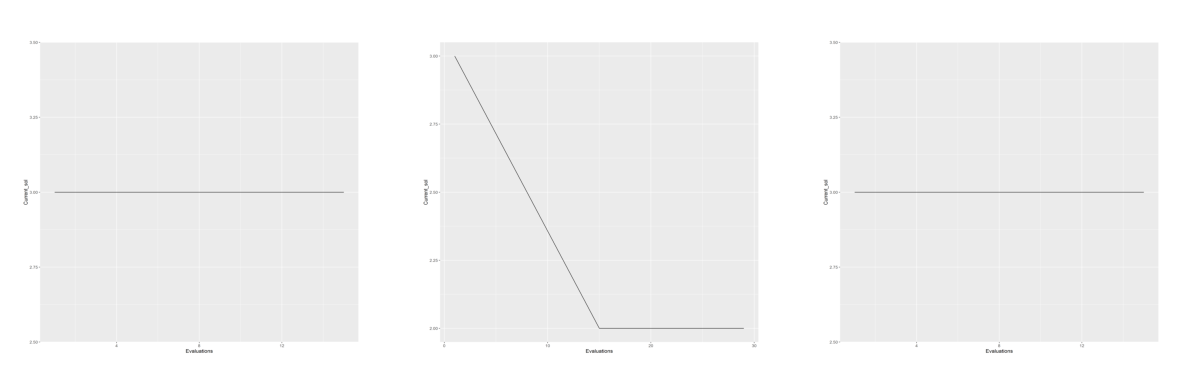
\includegraphics[width=\maxwidth]{figure/unnamed-chunk-12-1} \caption[Grafo handiak, Aging motakoak, hirugarren ingurunea erabilita]{Grafo handiak, Aging motakoak, hirugarren ingurunea erabilita}\label{fig:unnamed-chunk-12}
\end{figure}


\end{knitrout}
\end{center}
Emaitzak berdinak direla esan dezakegu, [3,2] artekoak. Baina gutxiagotan lortu dugu 2 balio duen soluzio bat. eta hobekuntza gutxiago gertatu dira  Aging grafo txikiekin konparatuta.\\

\begin{center}	
\begin{knitrout}
\definecolor{shadecolor}{rgb}{0.969, 0.969, 0.969}\color{fgcolor}\begin{figure}[!h]
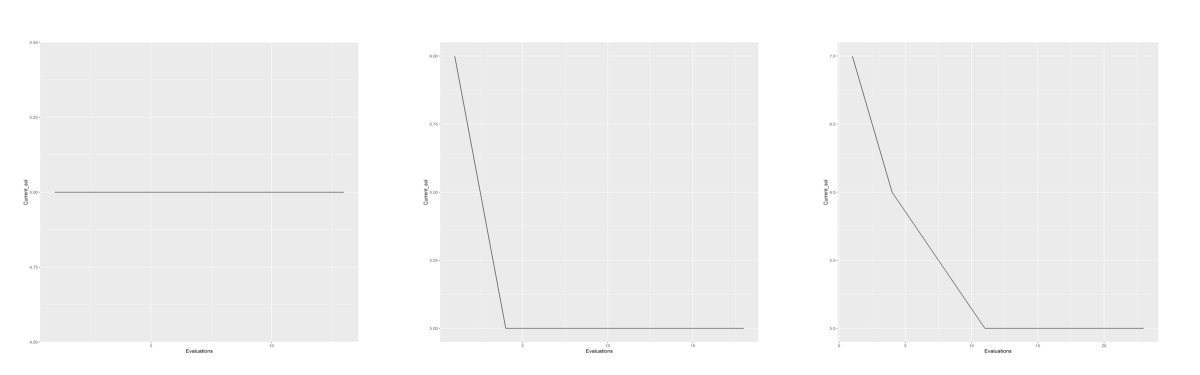
\includegraphics[width=\maxwidth]{figure/unnamed-chunk-13-1} \caption[Grafo handiak, Erdos motakoak, lehenengo ingurunea erabilita]{Grafo handiak, Erdos motakoak, lehenengo ingurunea erabilita}\label{fig:unnamed-chunk-13}
\end{figure}


\end{knitrout}
\end{center}


\begin{center}	
\begin{knitrout}
\definecolor{shadecolor}{rgb}{0.969, 0.969, 0.969}\color{fgcolor}\begin{figure}[!h]
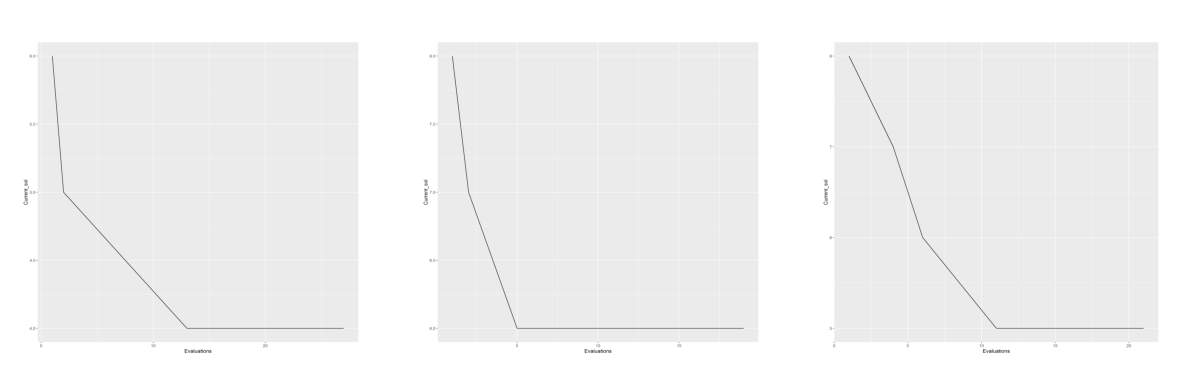
\includegraphics[width=\maxwidth]{figure/unnamed-chunk-14-1} \caption[Grafo handiak, Erdos motakoak, bigarren ingurunea erabilita]{Grafo handiak, Erdos motakoak, bigarren ingurunea erabilita}\label{fig:unnamed-chunk-14}
\end{figure}


\end{knitrout}
\end{center}


\begin{center}	
\begin{knitrout}
\definecolor{shadecolor}{rgb}{0.969, 0.969, 0.969}\color{fgcolor}\begin{figure}[!h]
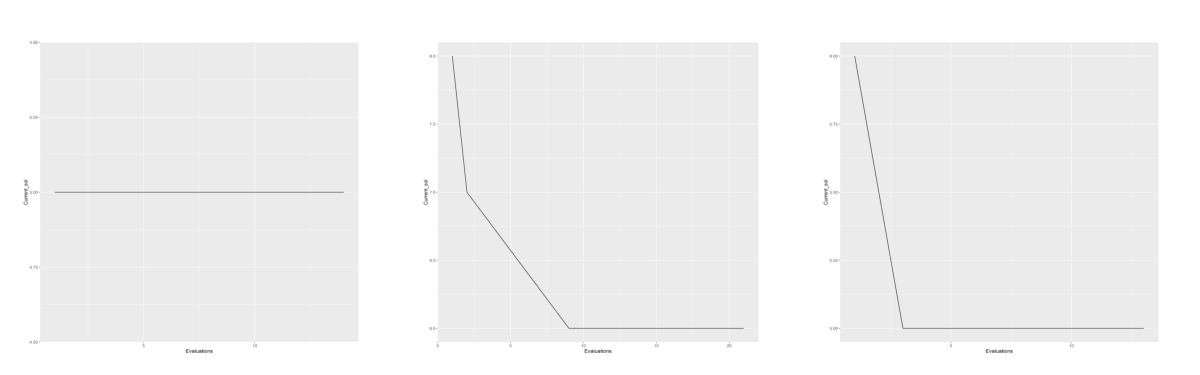
\includegraphics[width=\maxwidth]{figure/unnamed-chunk-15-1} \caption[Grafo handiak, Erdos motakoak, hirugarren ingurunea erabilita]{Grafo handiak, Erdos motakoak, hirugarren ingurunea erabilita}\label{fig:unnamed-chunk-15}
\end{figure}


\end{knitrout}
\end{center}
Hobekuntza ia beti gertatu da, gogoan izan grafo hauek 200 tamaina dutela eta soluzioaren luzeera 7 dela, honek soluzio posible gehiago eskaitzen ditu eta hobekuntza aukera gehiago ere, azken finean K = 7 ezarri dugu eta honek 2 zenbaki gehiagorekin soluzio posible berriak bilatzeko aukera ematen digu, soluzio espazioa txikietan baino askoz andiagoa izan arren.\\
Emaitzak 5-etik 4-era doaz (4 bakarra lortu da). Hasierako soluzioak ere aldatu egin dira 8-tik 5-era. \\

\begin{center}	
\begin{knitrout}
\definecolor{shadecolor}{rgb}{0.969, 0.969, 0.969}\color{fgcolor}\begin{figure}[!h]
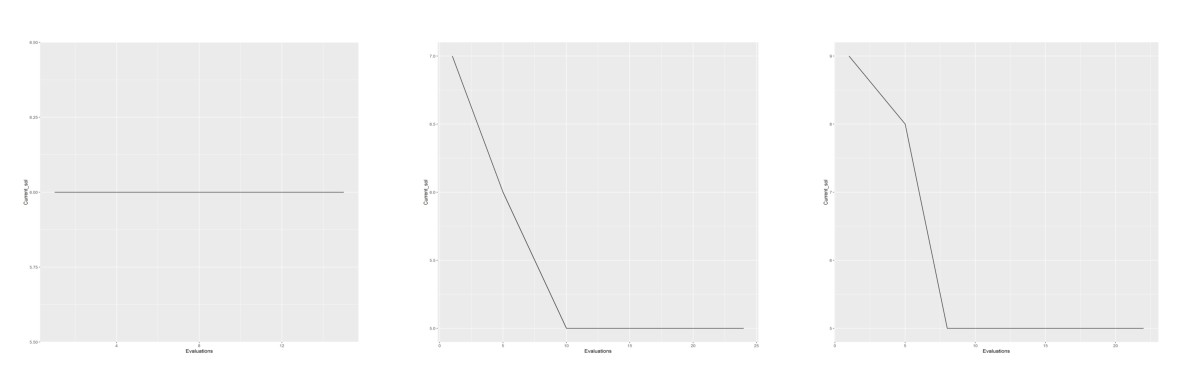
\includegraphics[width=\maxwidth]{figure/unnamed-chunk-16-1} \caption[Grafo handiak, Watts motakoak, lehenengo ingurunea erabilita]{Grafo handiak, Watts motakoak, lehenengo ingurunea erabilita}\label{fig:unnamed-chunk-16}
\end{figure}


\end{knitrout}
\end{center}

\begin{center}	
\begin{knitrout}
\definecolor{shadecolor}{rgb}{0.969, 0.969, 0.969}\color{fgcolor}\begin{figure}[!h]
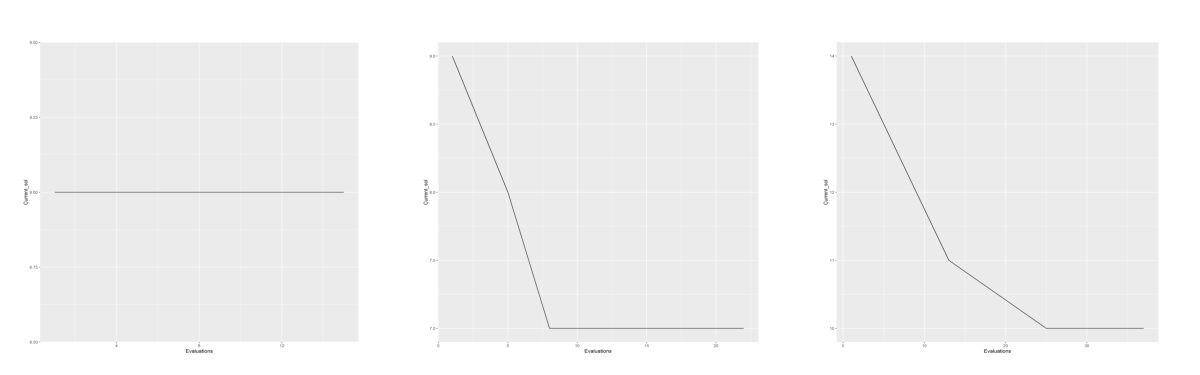
\includegraphics[width=\maxwidth]{figure/unnamed-chunk-17-1} \caption[Grafo handiak, Watts motakoak, bigarren ingurunea erabilita]{Grafo handiak, Watts motakoak, bigarren ingurunea erabilita}\label{fig:unnamed-chunk-17}
\end{figure}


\end{knitrout}
\end{center}

\begin{center}	
\begin{knitrout}
\definecolor{shadecolor}{rgb}{0.969, 0.969, 0.969}\color{fgcolor}\begin{figure}[!h]
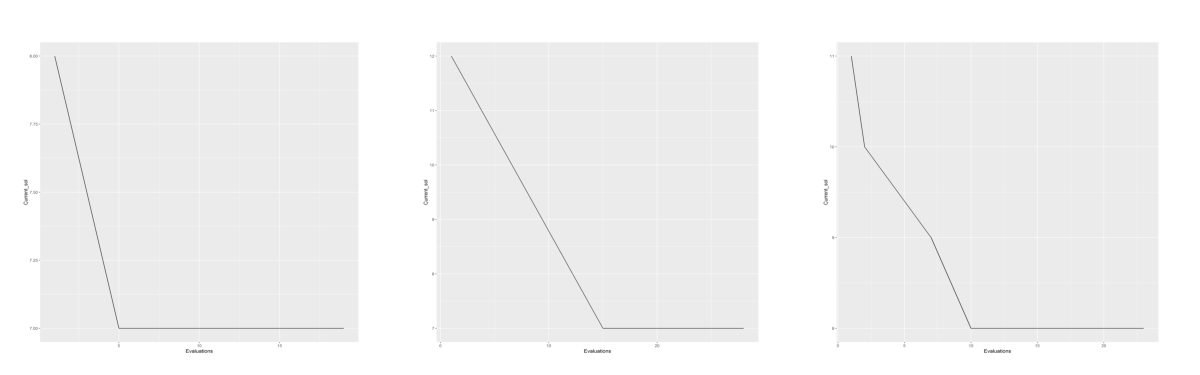
\includegraphics[width=\maxwidth]{figure/unnamed-chunk-18-1} \caption[Grafo handiak, Watts motakoak, hirugarren ingurunea erabilita]{Grafo handiak, Watts motakoak, hirugarren ingurunea erabilita}\label{fig:unnamed-chunk-18}
\end{figure}


\end{knitrout}
\end{center}

Kasu honetan optimoa 5 dela ikusi dezakegu, hirugarren inguruneak lortu duena, baina soluzioen balio anitzak somatu daitezke grafoetan, zenbaki altuetatik hasten direlako eta bazuetara jaisten direlako grafikoak. Adibidez hirugarren ingurunean ikusten den bezela, 12-tik 7-ra doa banan banan.\\


Obekuntza gertatzeko behar diren ebaluaketa kopurua desberdina dela ikus daiteke maldaren arabera, hau ingurunean dauden soluzioak eta hauen ordenaren araberakoak izango dira, obekuntza sortzen duen soluzio posiblea topatu arte.\\

Hiru grafo moten artean desberdintasun handia dagoela esan dezakegu. Lehengo grafo mota (Aging Ba Game) oso soluzio erraza duela esan dezakegu, beti 2 duelako optimotzat eta beti 2 edo 3 izango dugulako hasierako ausazko soluzioaren balioa. Bigarren grafo mota (Erdos Renyi Game) eta hirugarren grafo mota (Watts Strogatz Game)berriz, emaitza aniztasun handiagoa dute eta ikusitako soluzioak 10-etik 4-era joan daitezke Erdos grafo moten kasuan (5-era Watts grafo moten kasuan). Grafoen egitura eta mota oso garrantzitsua dela esan dezakegu, gehien bat holako proiektuak egiterako orduan.\\

Inguruneak ikusita, lehen eta bigarren inguruneak oso antzekoak direna ikusi dezakegu, azken finean 1 edo 2 gehitzea edo kentzea soluzioaren zenbaki bati ez da oso aldaketa handia. Baina hirugarren ingurunearekin obekuntza gehiago topatzen direla dirudi, emaitza optimoa guztietan ez topatu arren. Bi inguruneak batean batzea soluzio bakoitzaren bizilagun kopurua handitzen ditu, eta hobekuntza gertatzeko aukera ere.\\

Tamainen arteko ezberdintasunak topa daitezke, grafo handietan ingurune berdina izanda hobekuntza gehiago gertatzen direla ikusi daiteke. Hau soluzioen ingurunearen eta soluzio bakoitzaren neighborhoodaren araberakoa da. Soluzio posible gehiago izatean, hasierako soluzioa (Random) balio desberdinak errazago izatea ahalbidetzen du (Aging grafoak alde batera utzita). Honen ondorioz eta grafoaren tamainaren ondorioz soluzio bakoitzaren bizilagunen artean balio desberdinak errazago topatzea ahalbidetzen du. Honi K handitu dugula (K = 7) gehitu behar zaio  eta honek soluzio bakoitzari bizilagun gehiago izateko aukera eskaintzen dio, lehen eta bigarren inguruneak hirugarren ingurunearen alboan bezala. 

\pagebreak

\subsection{Algoritmo memetikoaren parametroen egokitzapena}
\paragraph{}Hainbat parametro dira algoritmo memetikoan aldatu daitezkenak, populazioaren tamaina, mutaketa indizea, bilaketa lokal mota eta bilaketa lokala izateko probabilitatea besteak bezte.\\

\subsubsection{Populazioaren tamaina}
\paragraph{}
Egin dugun lehenengo proba, populazioa aldatzea izan da. Lehenengo horrian tamaina txikiko grafo batean zortzi populazio desberdinekin egindako proben grafikoak daude.\\
\hspace*{1.2cm}\textbf{Grafoa:} Erdos Renyi game n=50 p=2/50\\
\hspace*{1.2cm}\textbf{Denbora:} 60s\\
\hspace*{1.2cm}\textbf{Bilaketa lokalak:} 0.05eko probabilitatearekin, hau da 20tik 1\\
 
Ebaluazio kopurua populazioarekin jaizten da, baita ere ikusi daiteke populazio txikiak konbergentizia azkarragoa dutela handiak baino, hau ematen den kasuan.\\

Grafo honetarako, bakarrik 20eko populazioa zuen exekuzioak lortu zuen 3 bailioko soluzio bat eta gainera populazioaren batazbestekoa konbergitu du.\\

Hala ere, posiblea litzateke populazio handiek denbora gehiago emanda soluzio hobeagoetara konbergitzea, esan nahi duena agian 20 eko populazioa baino soluzioa hobeak lortzen dira 40eko populazioarekin eta denbora gehiagorekin. Honegaitik bi proba egin ditugu populazio handiekin jarrera hau ikusteko asmoz, 60 eta 120 segundo proba baikoitzeko, hurrengo horrian ikusi daitzkenak. Ondorioz, esan genezake denbora bikoizteak, populazio handien konbergentzian lagundu arren ez dituzte soluzio hobeagorik aurkitu eta kostua merezi ez duela erabaki dugu.\\

\begin{center}	
\begin{knitrout}
\definecolor{shadecolor}{rgb}{0.969, 0.969, 0.969}\color{fgcolor}
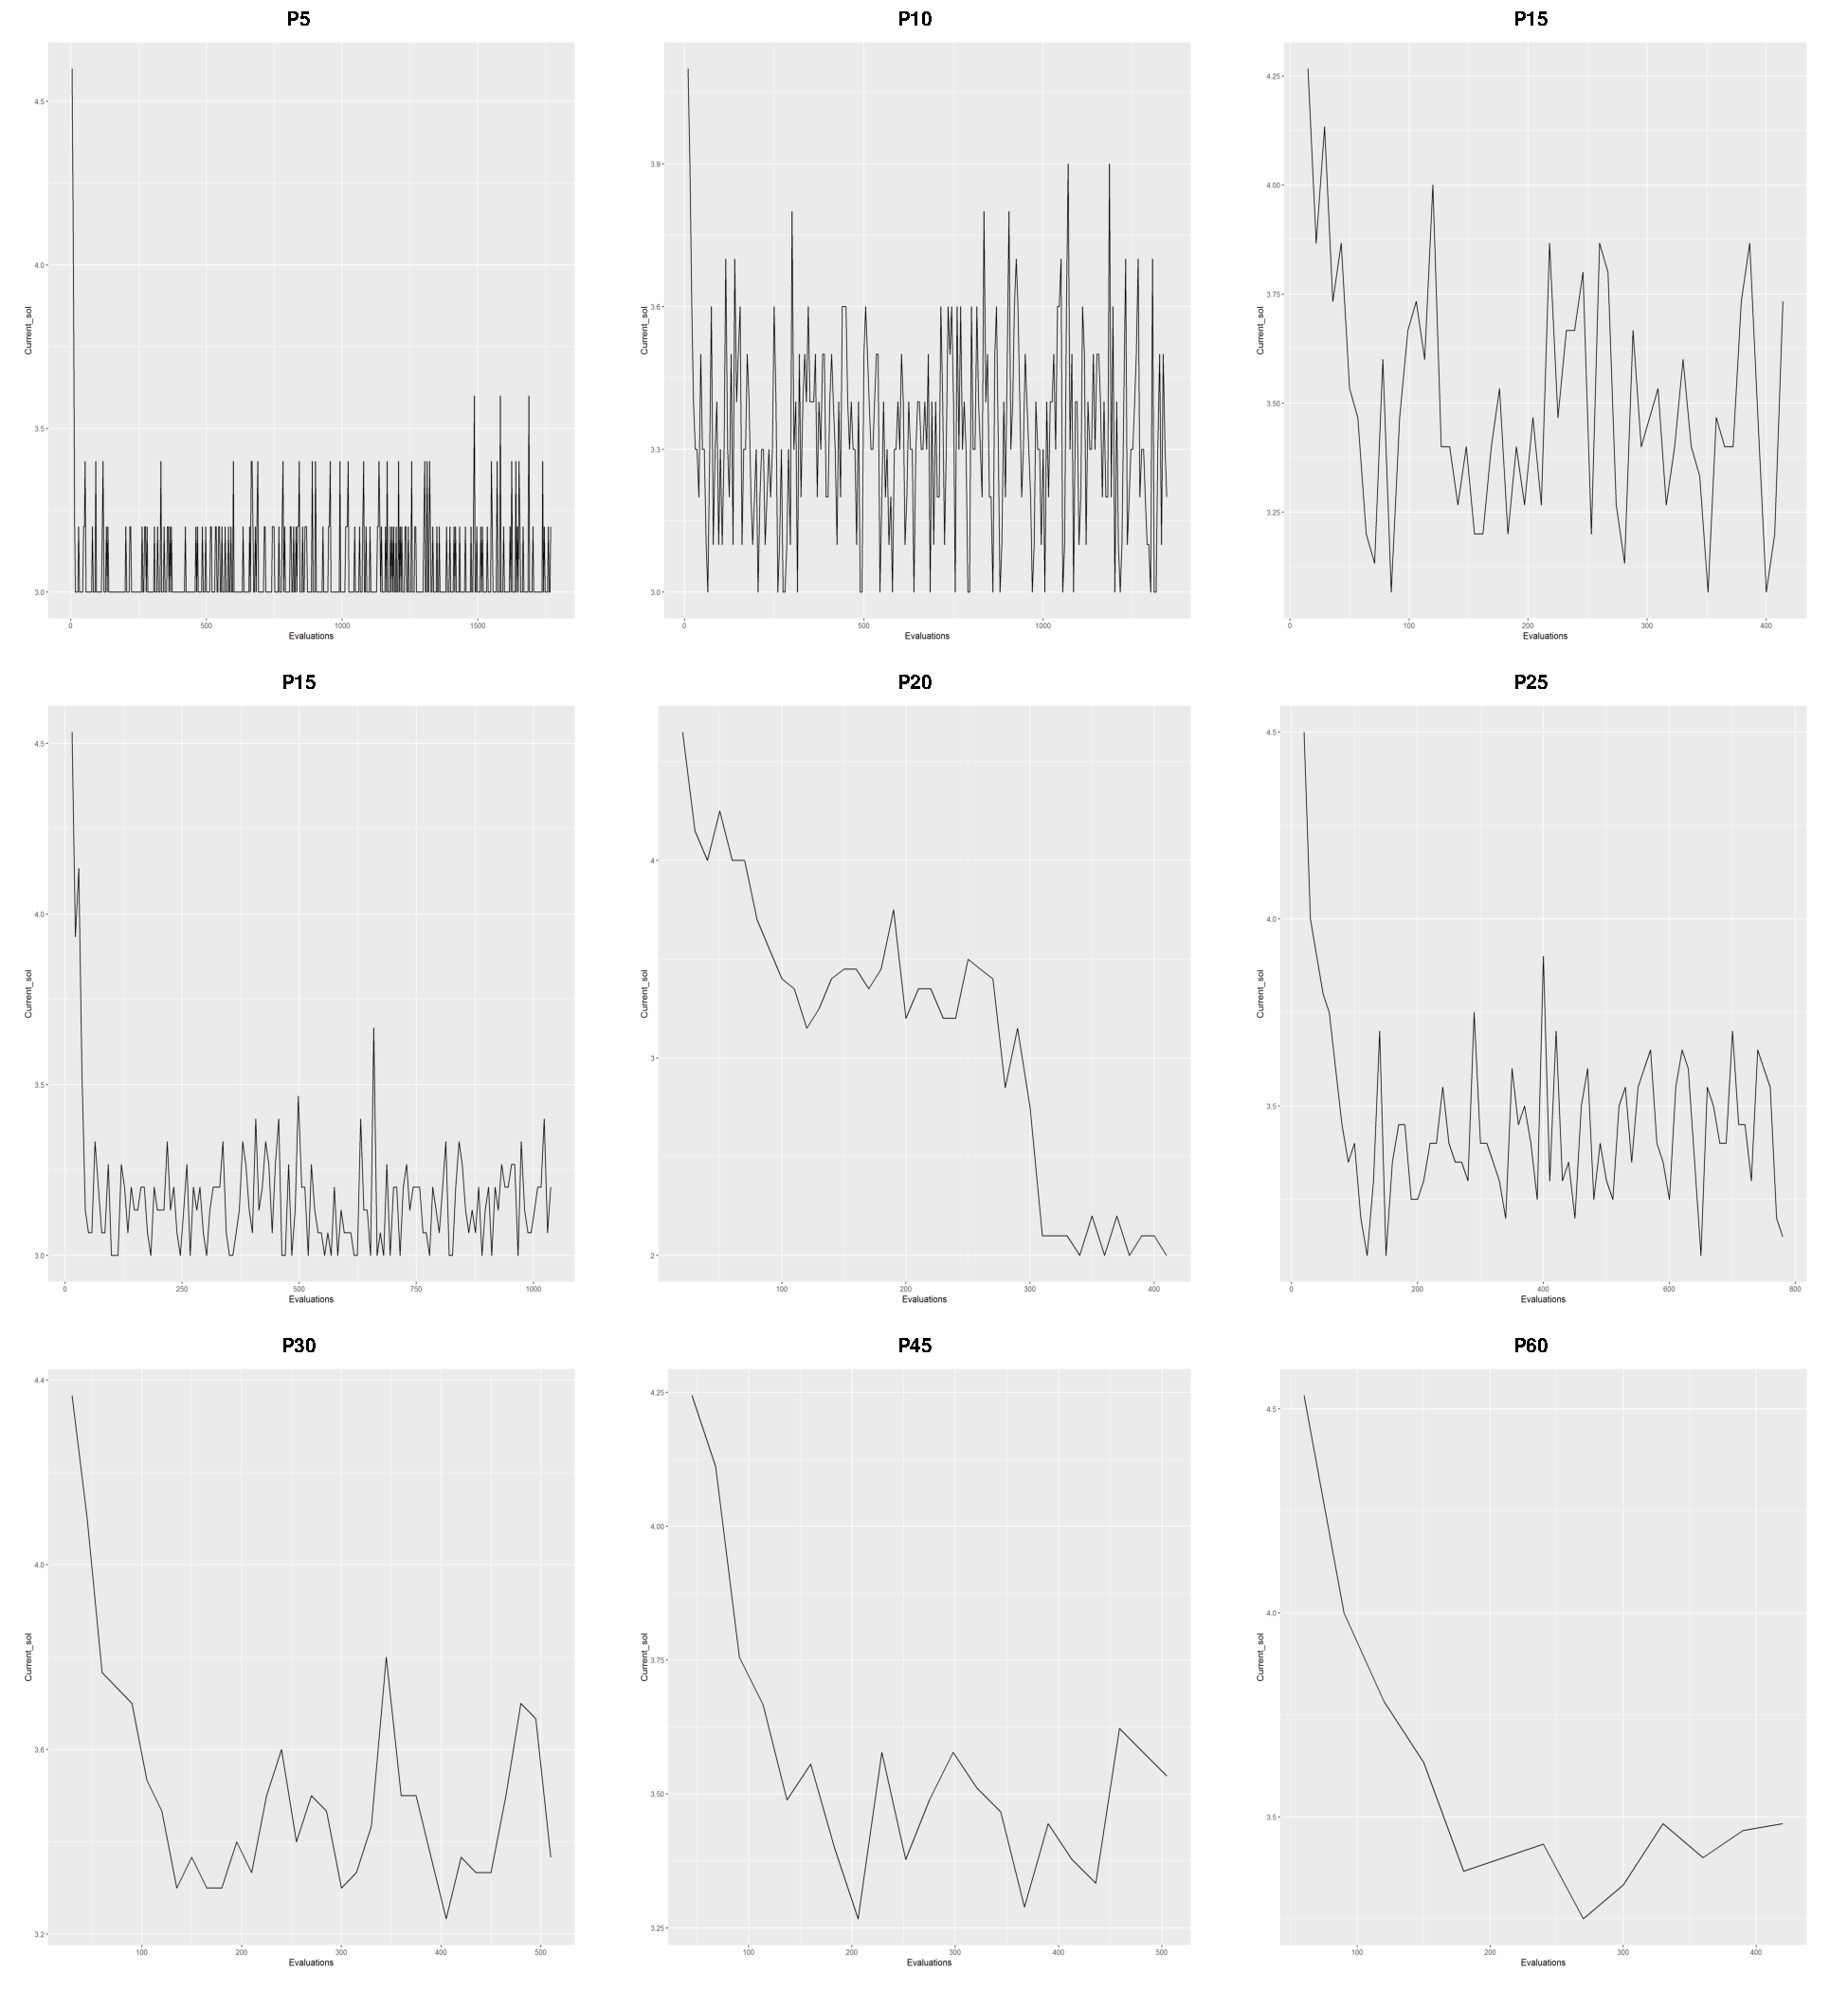
\includegraphics[width=\maxwidth]{figure/unnamed-chunk-19-1} 

\end{knitrout}
\end{center}

\begin{center}	
\begin{knitrout}
\definecolor{shadecolor}{rgb}{0.969, 0.969, 0.969}\color{fgcolor}
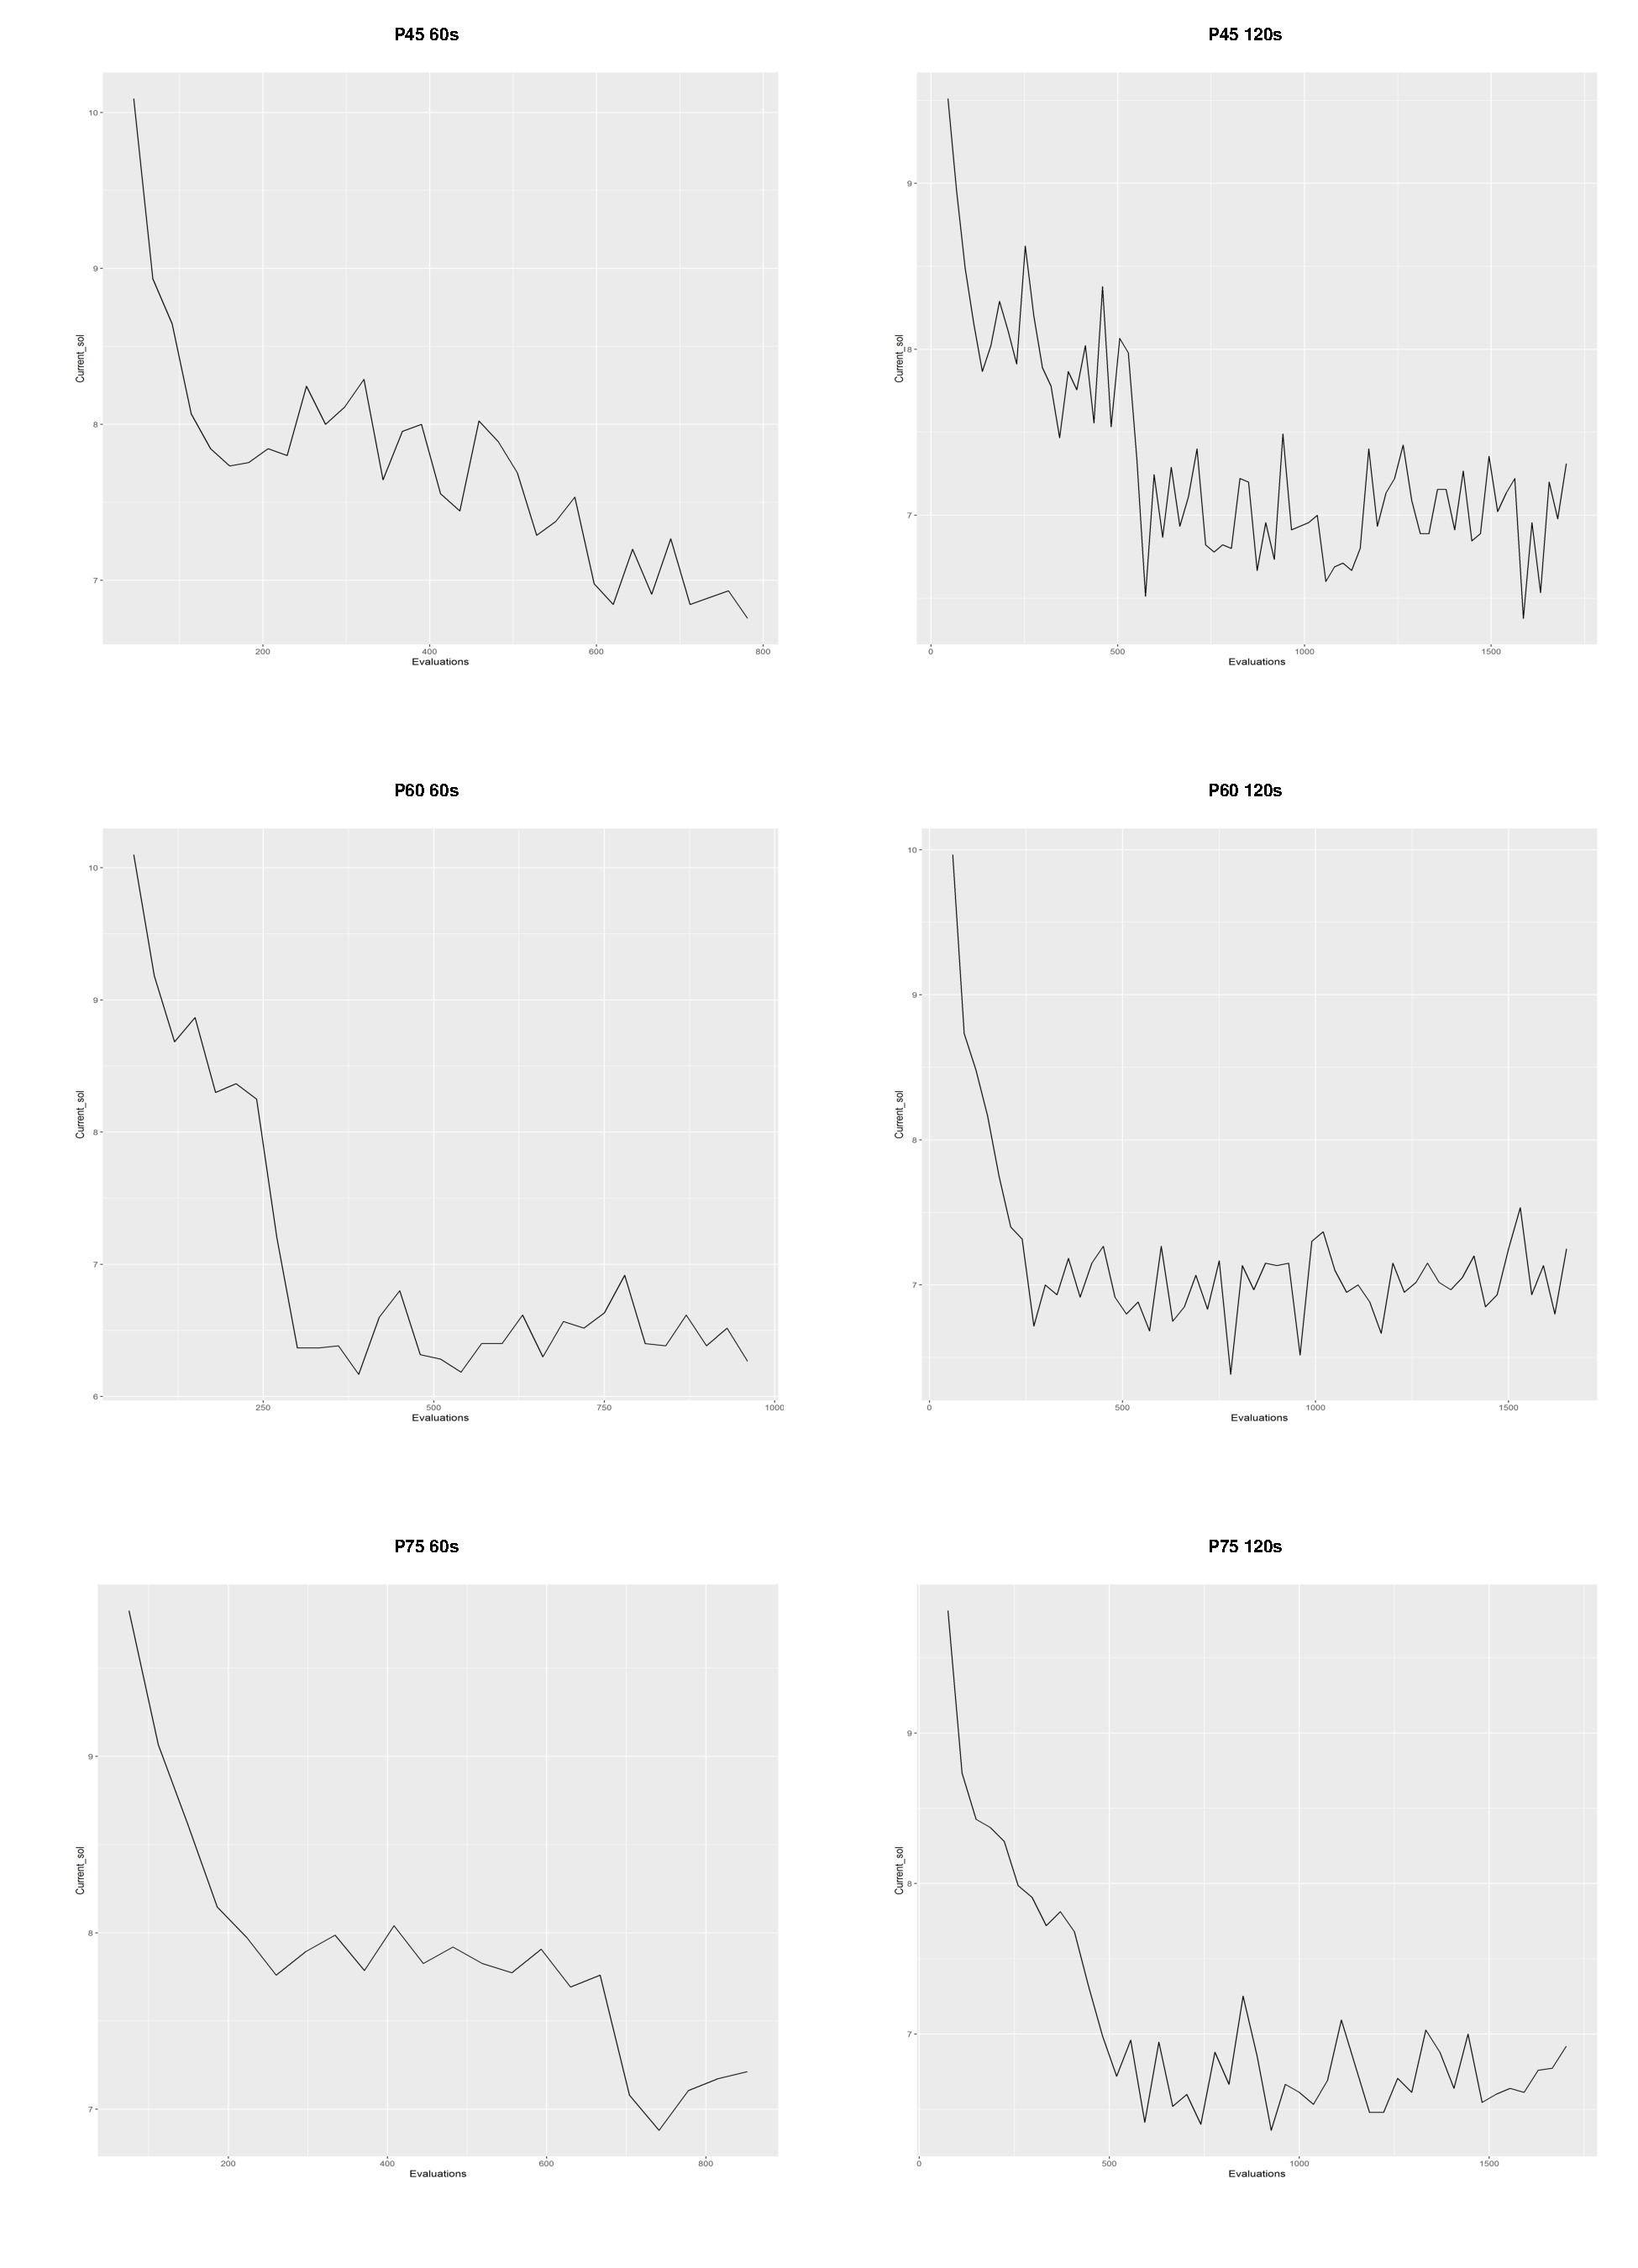
\includegraphics[width=\maxwidth]{figure/unnamed-chunk-20-1} 

\end{knitrout}
\end{center}

\pagebreak

\pagebreak
\subsubsection{Mutaketa parametroa}
\paragraph{}
Egin dugun bigarren proba, mutaketa parametroa aldatzea izan da, hona hemen tamaina txikiko grafo batean 8 populazio desberdinekin egindako proben grafikoak.\\
\hspace*{1.2cm}\textbf{Grafoa:} Watts strogatz game n=50 dim=1, nei=1, p=0.2\\
\hspace*{1.2cm}\textbf{Denbora:} 60s\\
\hspace*{1.2cm}\textbf{Bilaketa lokalak:} 0.05 p\\

Dakigun bezala, parametro honen egokitzapen zuzena oso garrantsitzua da, 1 izanda auzasko bilaketa bat bihurtuko genuke algoritmoa(Geure kasuam gen bakar bat mutatzen da beraz ez litzateke hau gertatuko) baina ideai hori da, populazioaren egokitzapena sahieztea. \\

Aurrez espero genuen 0.01 mutaketa ratioarekin aldaketa txikiak baina hala era ikusi dira eta hau bilaketa lokalaerengaitik izan beharko zen. Beztalde, bezte mutaketa balioek espero genuen portaera izan dute, non populazioaren egokitzapenean aldaketa gero eta haniagoak somatzen dira.\\

Parametro egokiena hautazearren, 0.1 eta 0.05 bailioetariko bat hautatzea erabaki genue, 20etik 2 edo 1 mutatzea. Askenean 0.05 erabiltzea erabaki dugu.\\


\begin{knitrout}
\definecolor{shadecolor}{rgb}{0.969, 0.969, 0.969}\color{fgcolor}
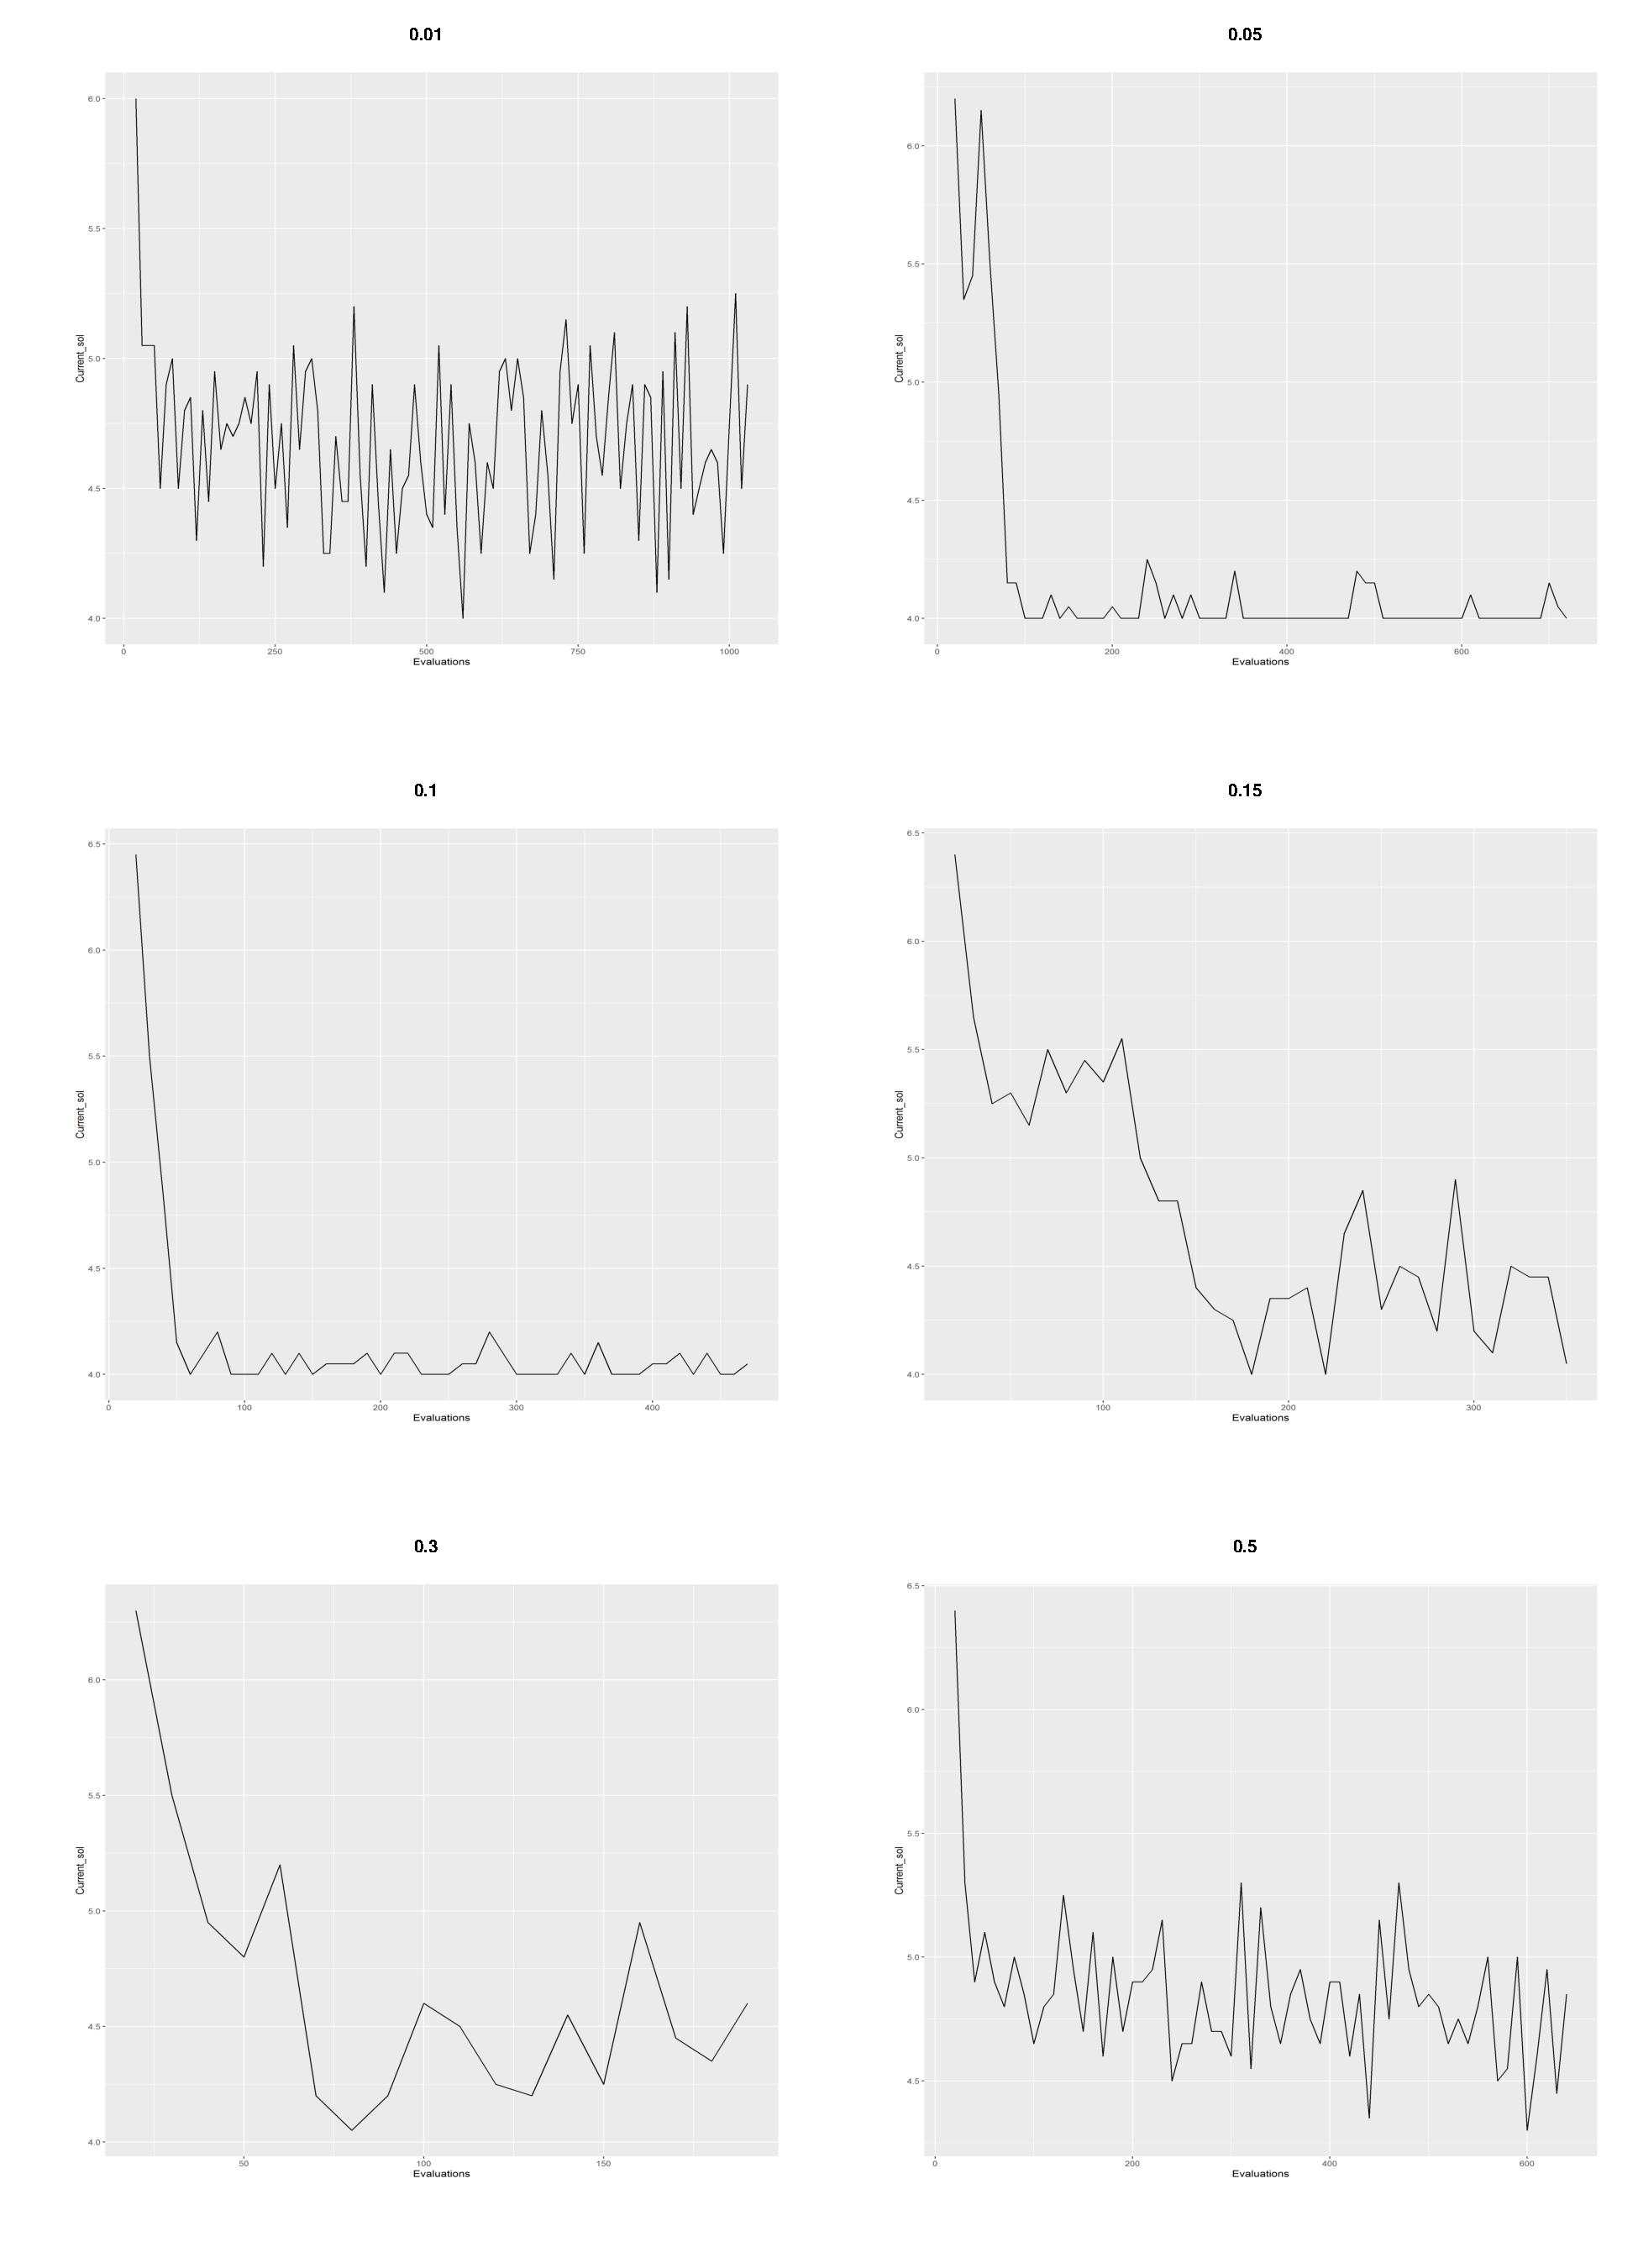
\includegraphics[width=\maxwidth]{figure/unnamed-chunk-21-1} 

\end{knitrout}

\end{center}

\subsection{Algoritmoen konparaketa}
\paragraph{}
Hurrengo histogramak, grafo bakoitzeko, algoritmo desberdinek aurkitutako soluzio hoberenen batazbeztekoak erakusten ditu. Lehenengo grafoetan, algoritmo guztiek soluzio berdia ematen dute, bai txikietan bai handietan. Grafoak sortzeko parametroak aldatu arren ez dugu lortu Watts grafoetan lortzen diren bezalako soluzioak. Azkeneko grafo hauken, kate egitura dute, eta iteresgarriak dira gure problemarako eta algoritmoen eraginkortasuna neurtzeko.\\

Igarri, histograman, altuerak batezbesteko soluzioen balio dela, honek dio altuagoa bada, txarragoa dela grafo horretarako.\\

Lortutako emaitzak esan bezala ez dira oso esanguratzuak, eta errore barrak ikusten ez diren arren ez zegoen ia desbiderapenik kasu gehienetan. Esan genezake, emaitzak ez direla nahikoa algoritmo bat bezteak baino hobeago denik baieztatzeko.\\

\begin{center}
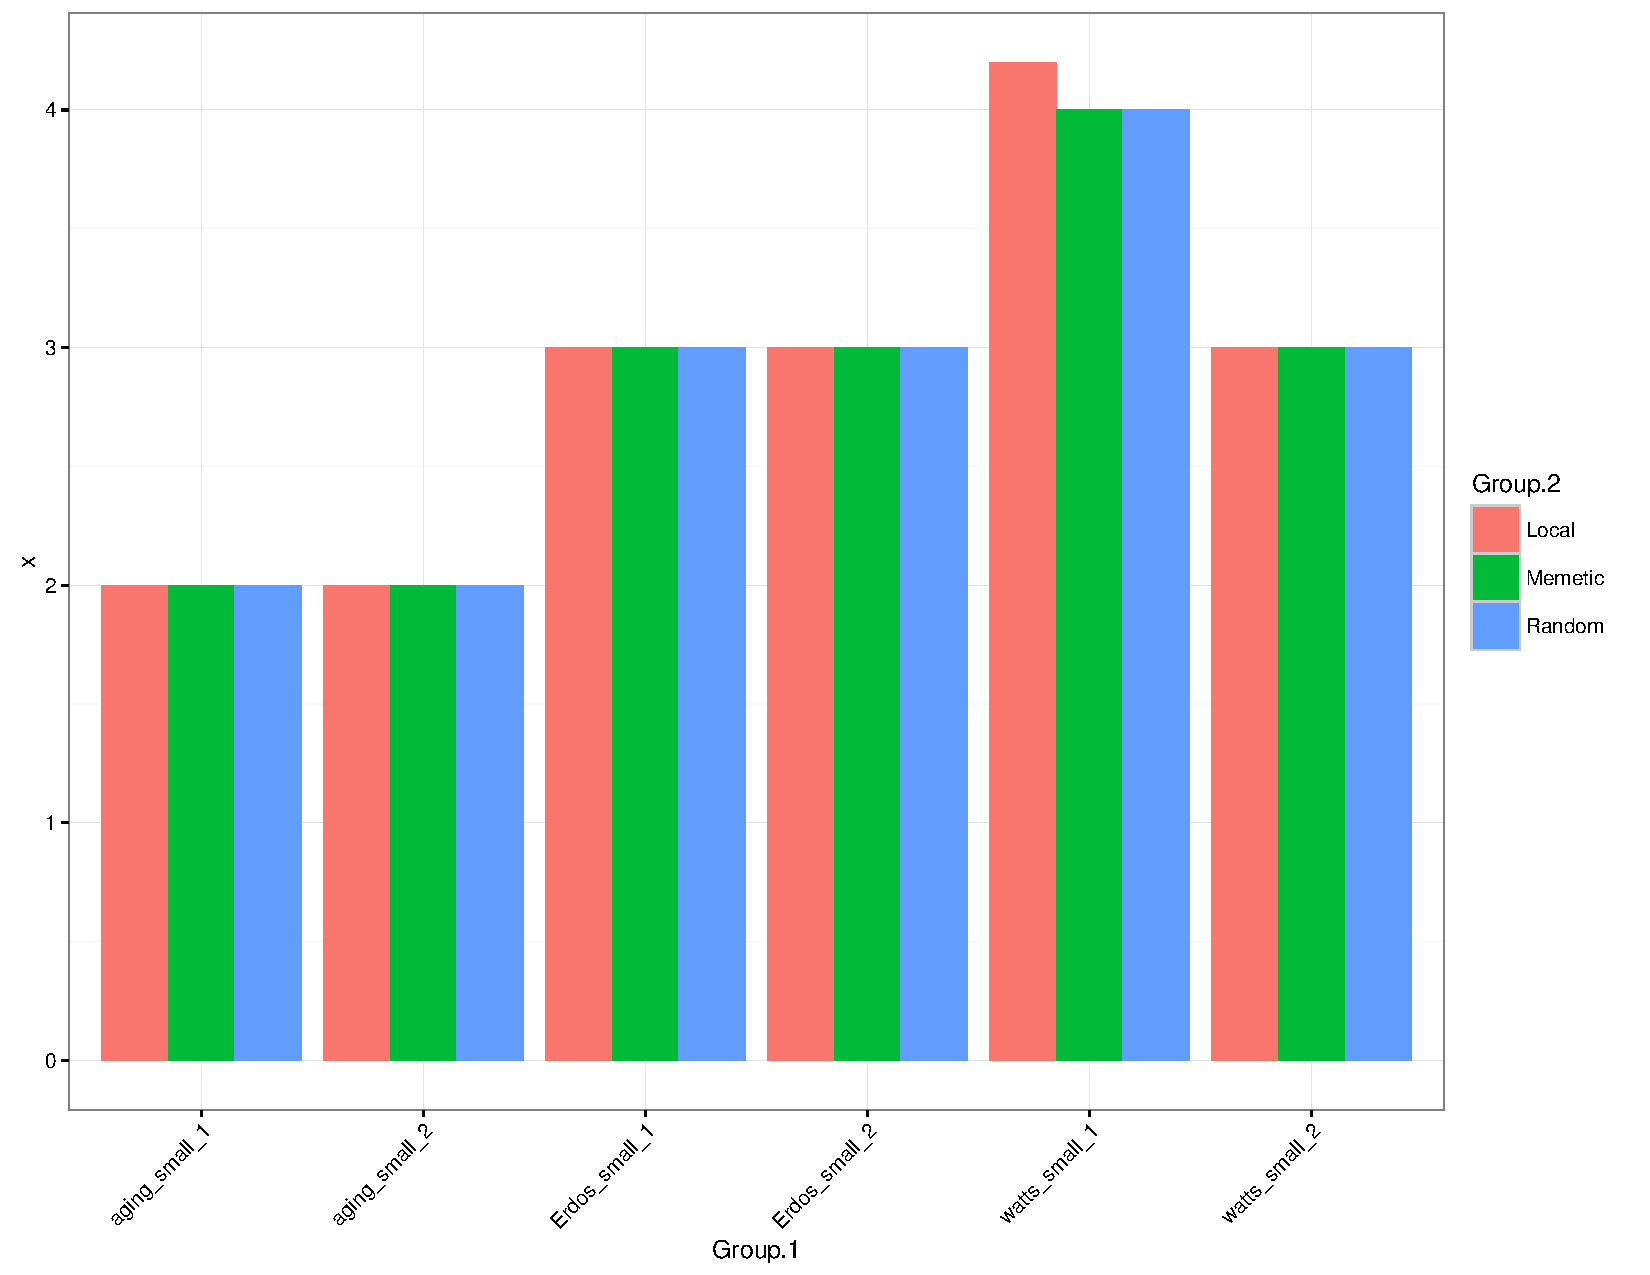
\includegraphics[scale=0.6]{HistoSmall.pdf} 
\end{center}
\pagebreak

\begin{center}
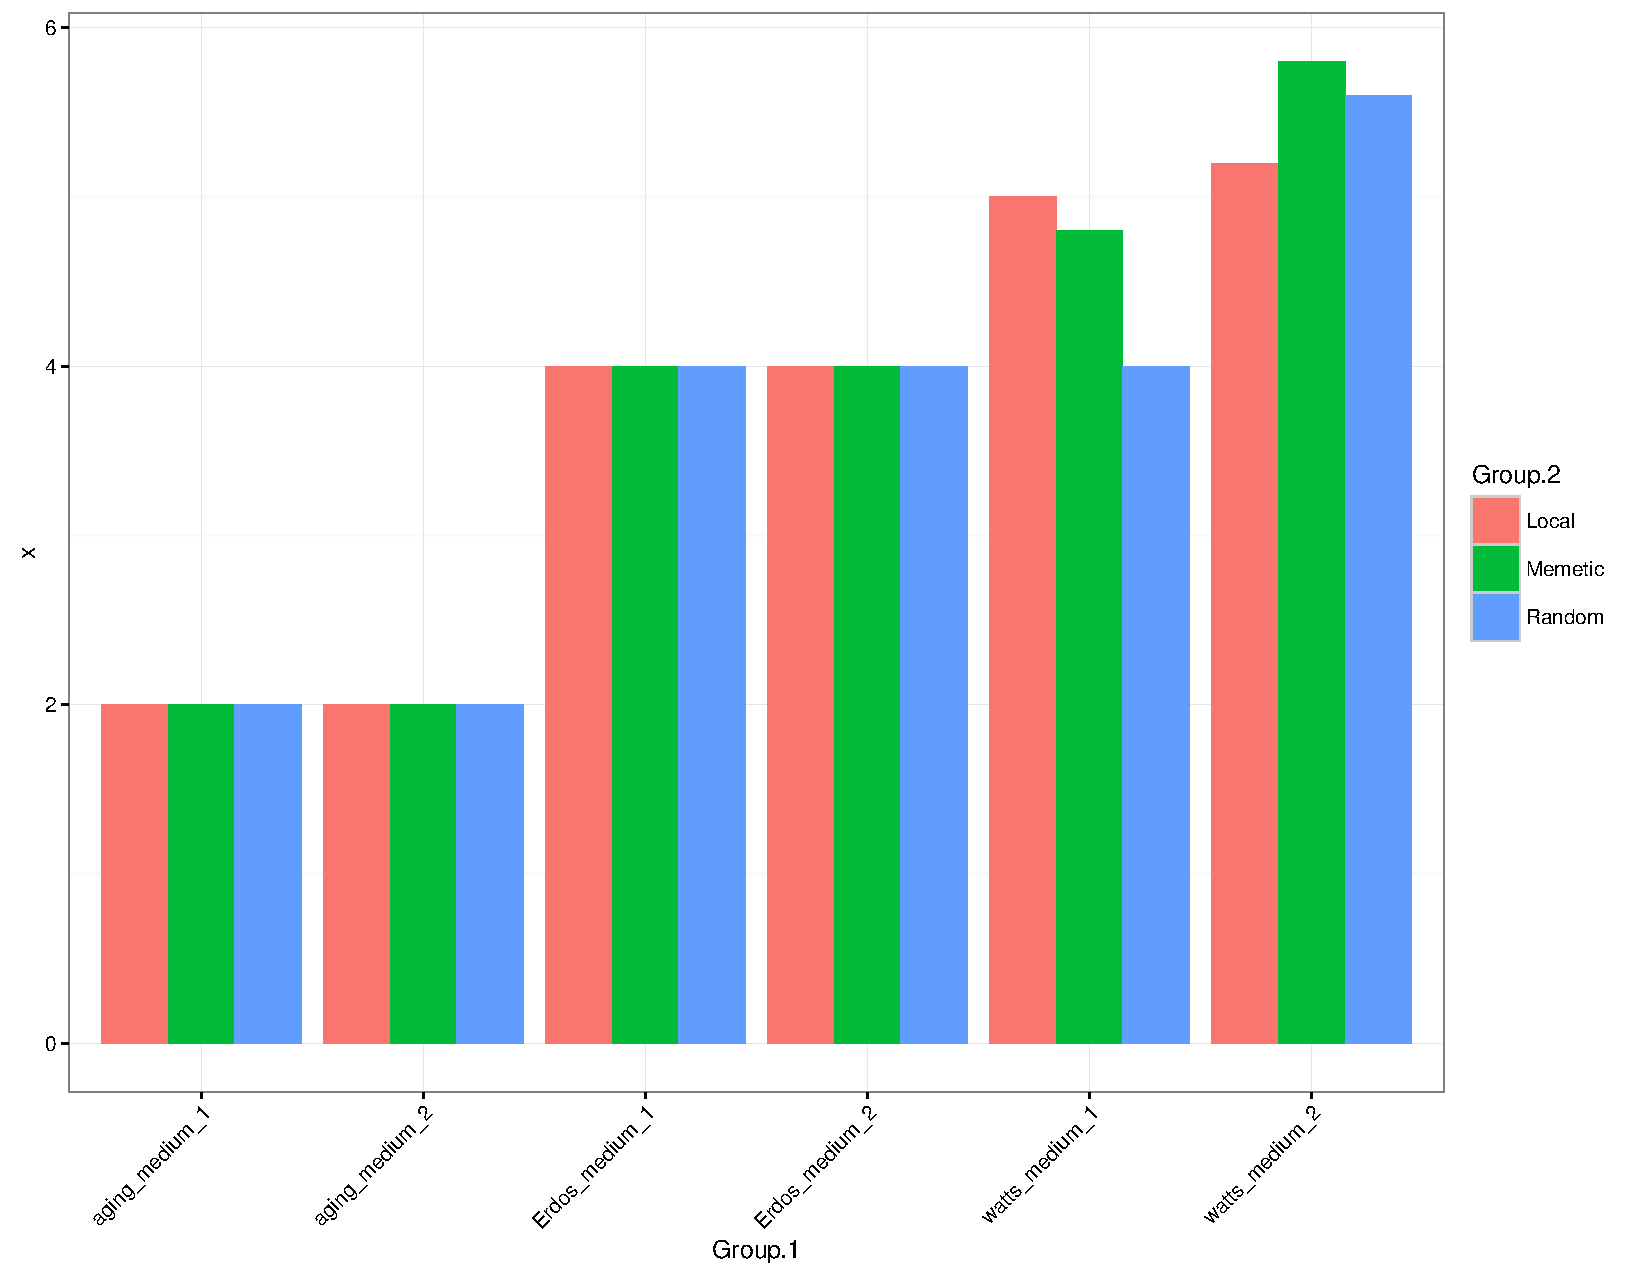
\includegraphics[scale=0.6]{HistoBig.pdf} 
\end{center}
\\

\subsection{Aurkitutako arazoak}
\paragraph{}
R programak, grafo eta parametro berdinak erabilita, exekuzio desberinetan ebaluazio kopuruan aldaketa handiak somatu ditugu, batzuetan programa oso askar hasi arren, oso motel bukatzen du, R “blokeatu” harte kasu batzuetan.\\

Arazo hau dela eta, bakarrik erabiliko diren programak eta grafoak sortu egiten genituen gure Worckspace-aren tamaina txikiagotzeko azkarrago exekuta dezan. Baita ere programen exekuzio bitartean ordenagailuaren beste aplikazioen erabilera murriztu egin dugu.\\


%%load("E:/Documentos/BilaketaHeuristikoak/MidTermExamLatex/BilaketaHeuristikoak_Ar2.8.R")
\end{document}
